\documentclass{article}

% Packages
\usepackage{amsmath}    
\usepackage{amsfonts}  
\usepackage{amssymb}    
\usepackage{graphicx}   
\usepackage{hyperref}   
\usepackage{booktabs}  
\usepackage{geometry}   
\usepackage{natbib}     
\usepackage{authblk}    
\usepackage{subcaption}
\usepackage{xcolor}
\usepackage{siunitx}
\usepackage{float}


\geometry{left=25mm, right=25mm, top=25mm, bottom=25mm}
\newcommand{\reddashedline}{\textcolor{red}{---}}
\newcommand{\orangedashedline}{\textcolor{orange}{---}}
\newcommand{\yellowdashedline}{\textcolor{yellow}{---}}
\newcommand{\greendashedline}{\textcolor{green}{---}}
\newcommand{\bluedashedline}{\textcolor{blue}{---}}
\newcommand{\purpledashedline}{\textcolor{purple}{---}}
\newcommand{\cyandashedline}{\textcolor{cyan}{---}}
\newcommand{\magentadashedline}{\textcolor{magenta}{---}}
\setlength{\parindent}{0pt}


\title{Planetary Mission}

\begin{document}
	
	
\section{Introduction}
The  PoliMi  Space  Agency  wants  to  launch  a  Planetary  Explorer  Mission,  to  perform  Earth Observation. This section carries out relevant orbital analysis and groundtrack estimation while also considering two perturbation models. A modified groundtrack was proposed for a repeating groundtrack, and two propagation methods are used to perform the analysis which are then compared. A comparison between the real data of a satellite and its analytical results obtained with the code model is also performed for model validity. 

\subsection{Nominal Orbit}

From the provided orbital parameters this satellite heavily contains geosynchronous orbital characteristics. Hence, the altitude at perigee is chosen as 35786 km - where it is possible to see the moon and J2 perturbation effect. $\Omega$ (right ascension of ascending node, $\omega$ (argument of perigee), and $f_0$ (initial true anomaly) are chosen arbitrarily for a simpler analysis.

%citation for GSO: https://www.esa.int/ESA_Multimedia/Images/2020/03/Geostationary_orbit

\begin{table}[ht]
	\centering
	\label{tab:keplerian_elements}
	\begin{tabular}{|c|c|c|c|c|c|}
		\hline
		a [km] & e [-] & i [°] & $\Omega$ [°] & $\omega$ [°] & altitude at perigee [km] \\
		\hline
		42159 & 0.0007 & 32.5934 & 0 & 85 & 35786 \\
		\hline
	\end{tabular}
	\caption{Keplerian elements of the orbit.}
	\label{tab:keplerian_elements}
\end{table}

The unperturbed nominal orbit is propagated as below in the Earth-centered reference frame:


\begin{figure}[H]
	\centering
	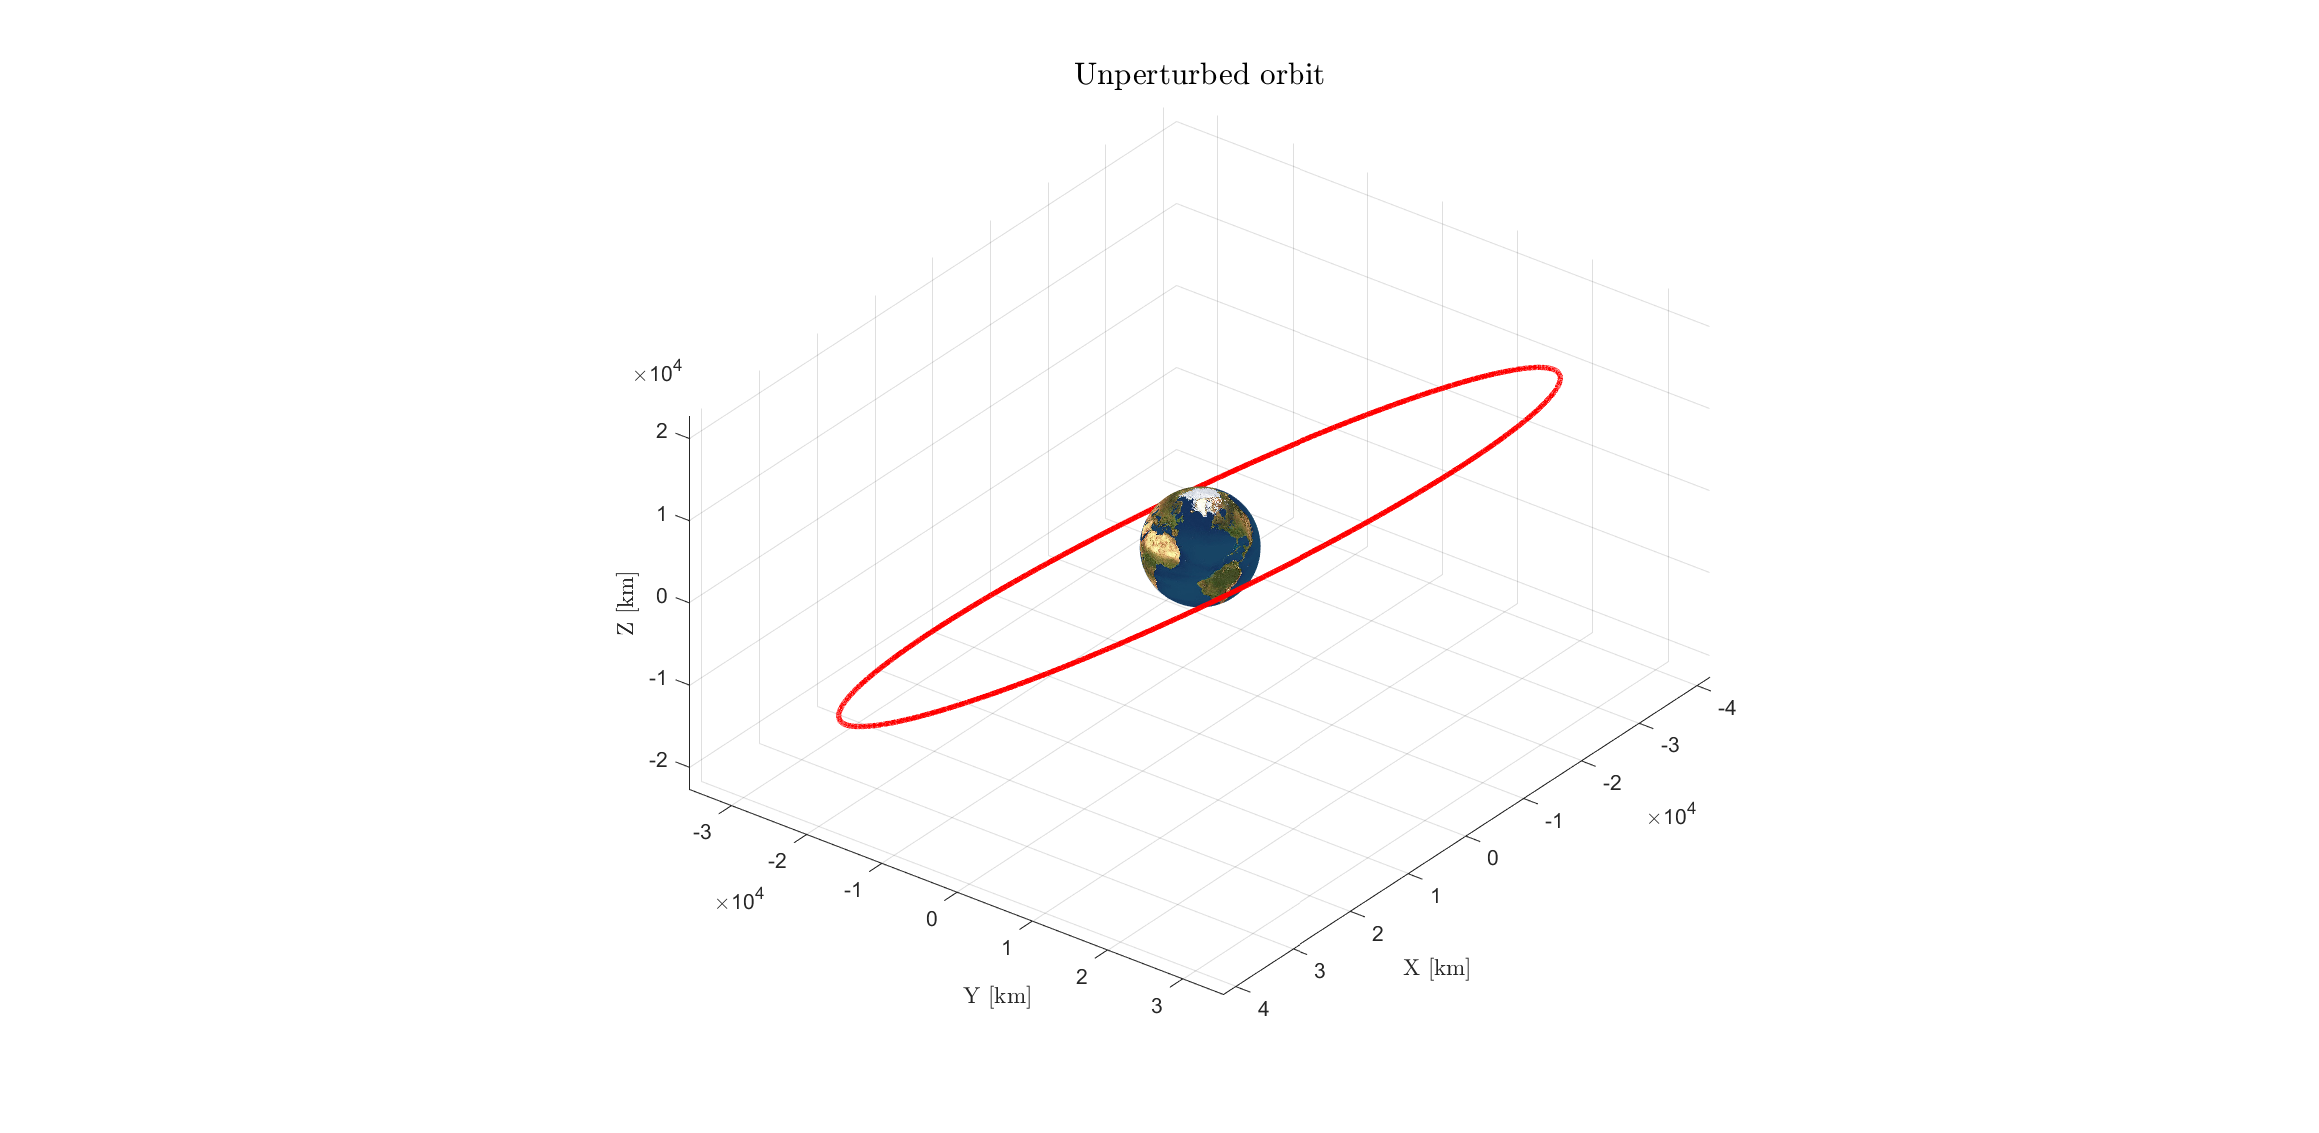
\includegraphics[width=0.8\textwidth]{nominal_orbit.eps}
	\caption{Assigned orbit.}
	\label{fig:nominal_orbit}
\end{figure}

\section{Groundtrack}
The satellite's orbit is propagated to compute its groundtrack. The motion of the spacecraft is assumed to be a perturbed two body problem in Cartesian coordinates, described by the equation:
\[
\dot{\mathbf{r}} = -\frac{\mu}{r^3} \mathbf{r} + \mathbf{a}_{\text{perturbation}}
\]
This is solved using Matlab's multi-step solver \texttt{ode113} function which is based on the Adams-Bashforth-Moulton method; it's chosen for its high accuracy over an extended period. A relative tolerance of \(1 \times 10^{-12}\) and absolute tolerance of \(1 \times 10^{-12}\) were selected for more precision.

%citation for formula: Curtis

\subsection{Unperturbed Groundtrack}
\subsubsection{Nominal Orbit Groundtrack}

The first required analysis of the ground track is for the nominal orbit considering an unperturbed case, where the $\mathbf{a}_{perturbation}$ in equation is null. The ground track was propagated for a period of 1 orbit of the satellite, 1 day and 10 days, as shown below.\\
\begin{figure}[H]
	\centering
	% First row with two figures
	\begin{subfigure}[b]{0.45\textwidth}
		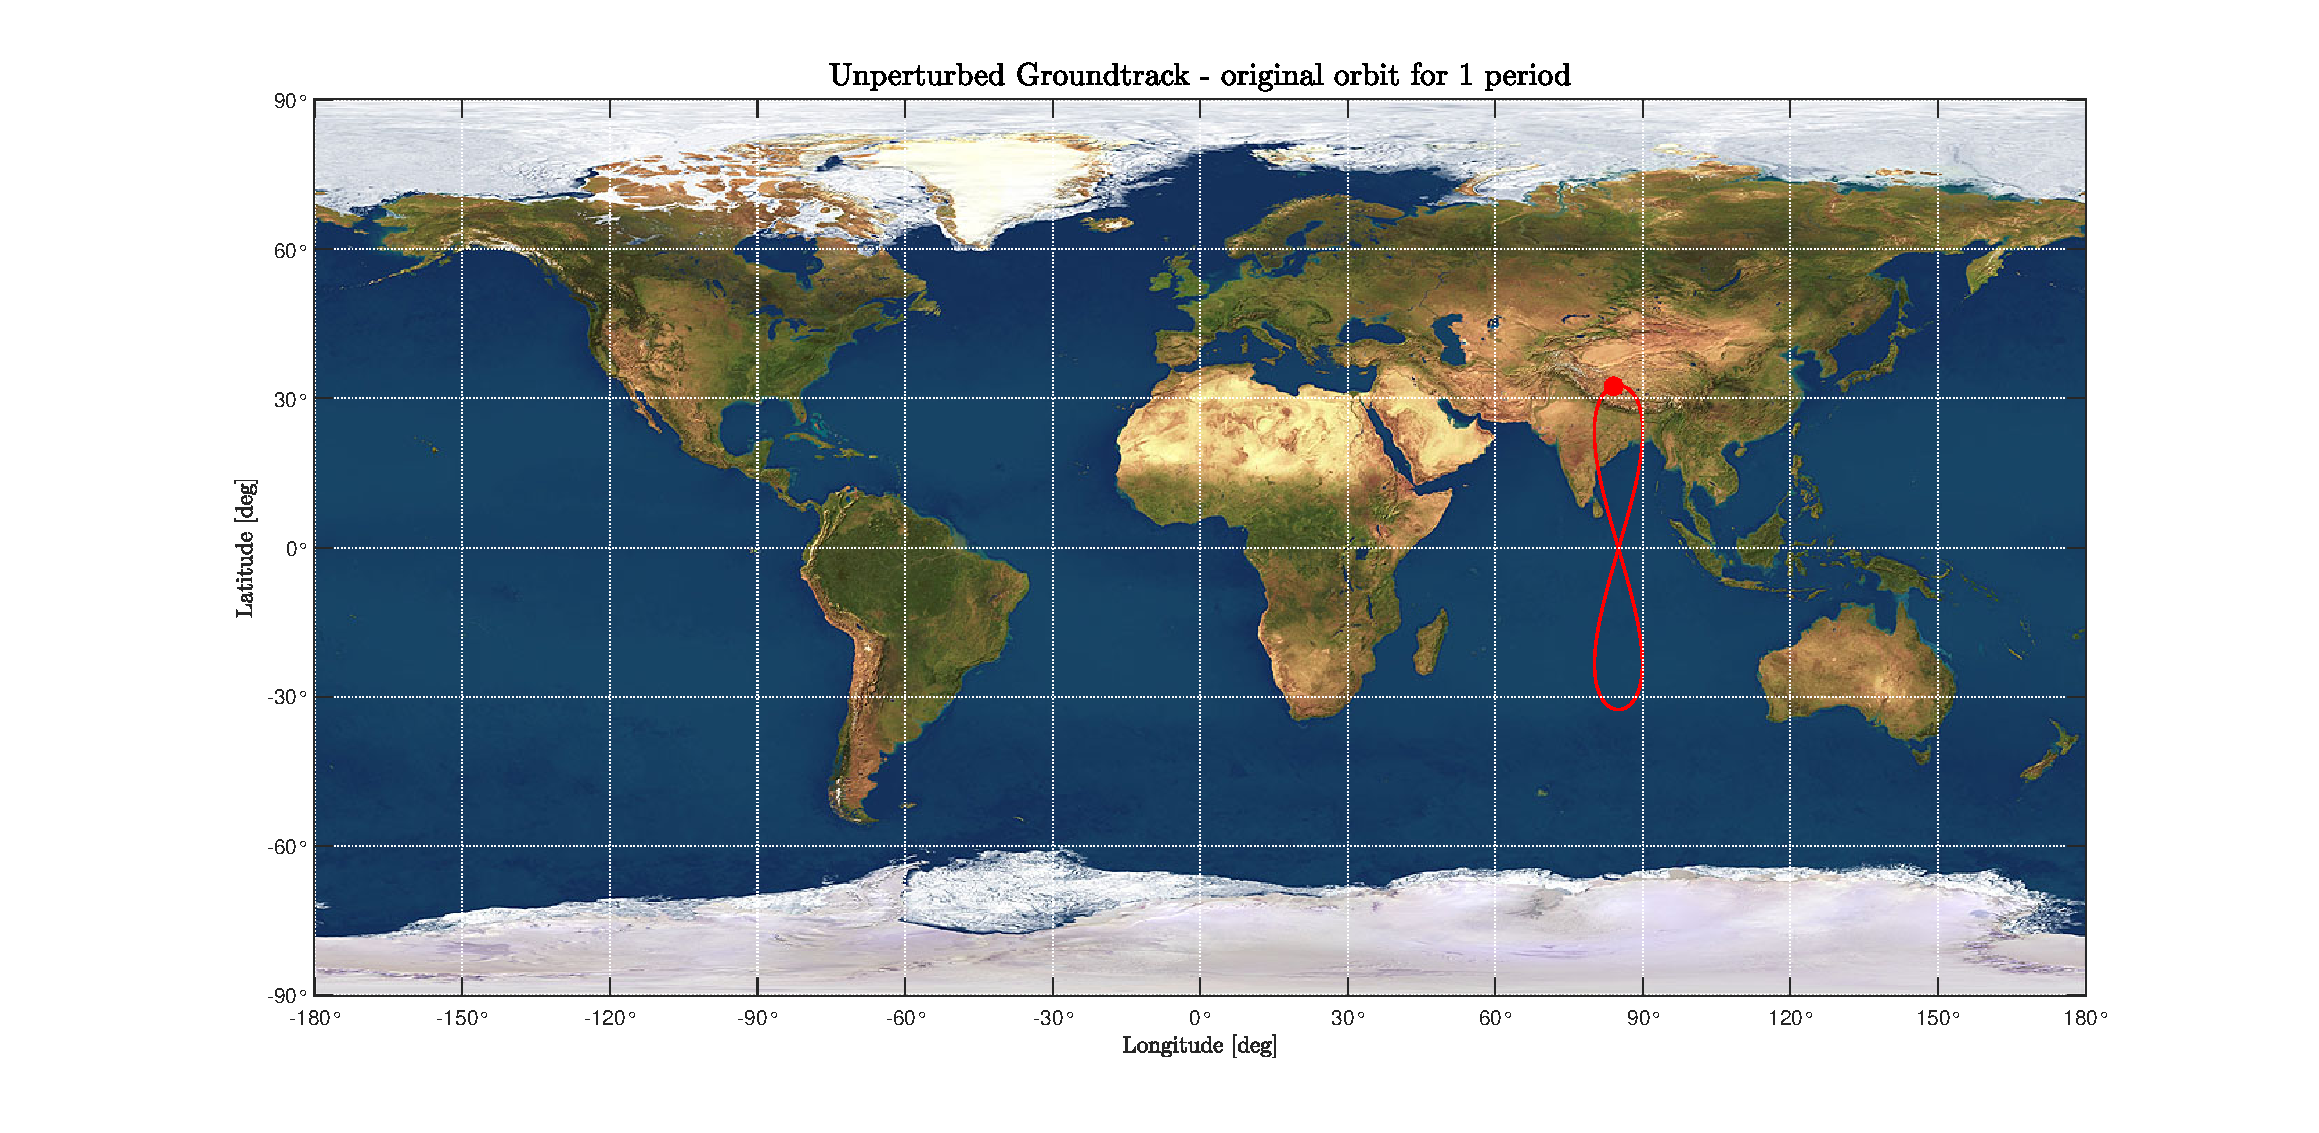
\includegraphics[width=\textwidth]{ug1orb.eps}
		\caption{}
		\label{fig:1a}
	\end{subfigure}
	\hfill
	\begin{subfigure}[b]{0.45\textwidth}
		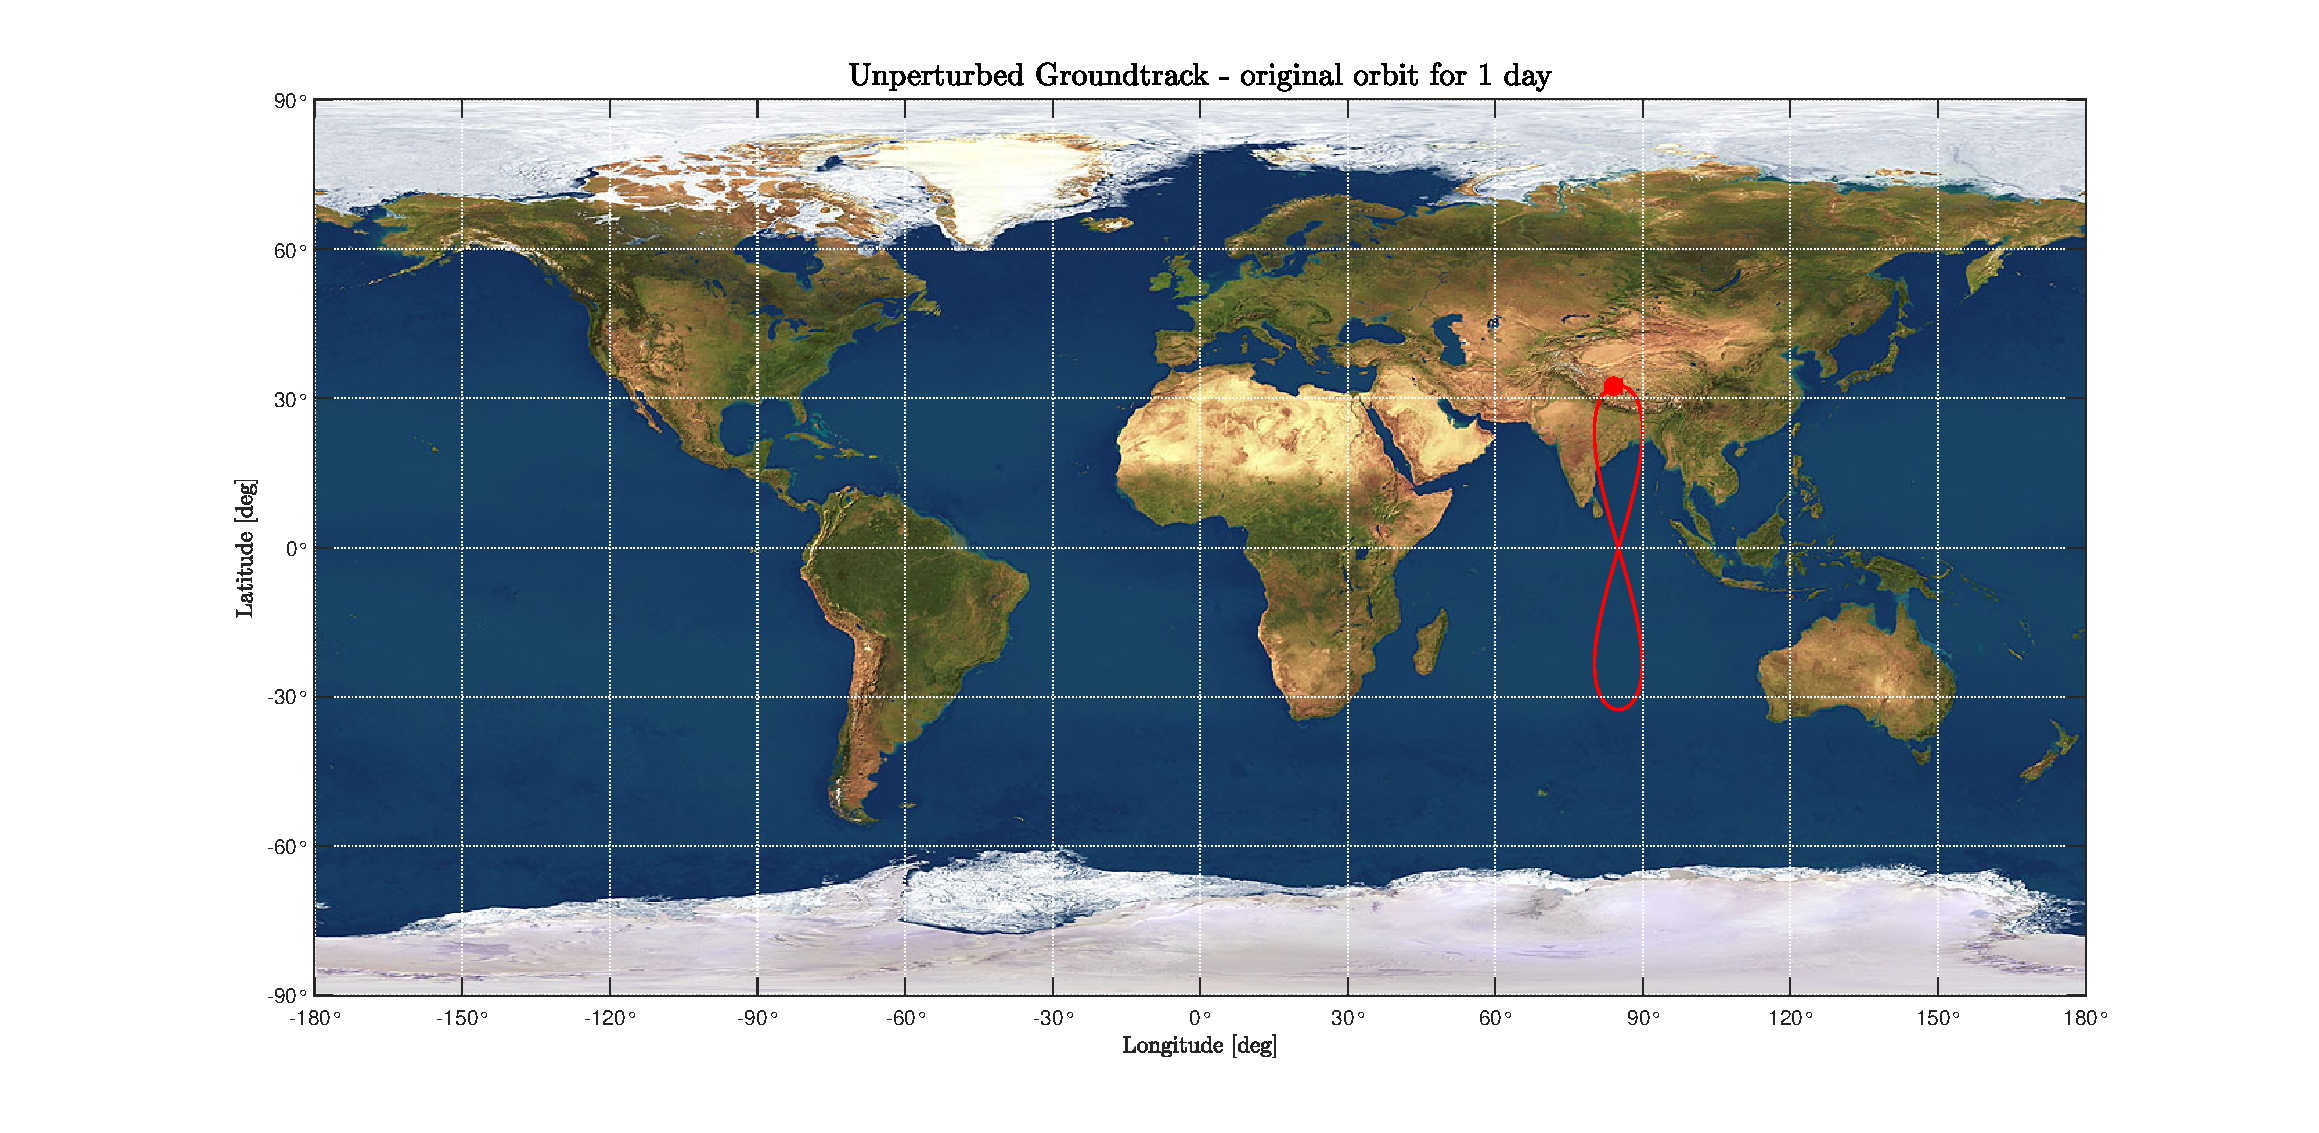
\includegraphics[width=\textwidth]{ug1d.eps}
		\caption{}
		\label{fig:1b}
	\end{subfigure}
	
	% Second row with two figures
	\vspace{1cm} % Adjust the vertical spacing as needed
	\begin{subfigure}[b]{0.45\textwidth}
		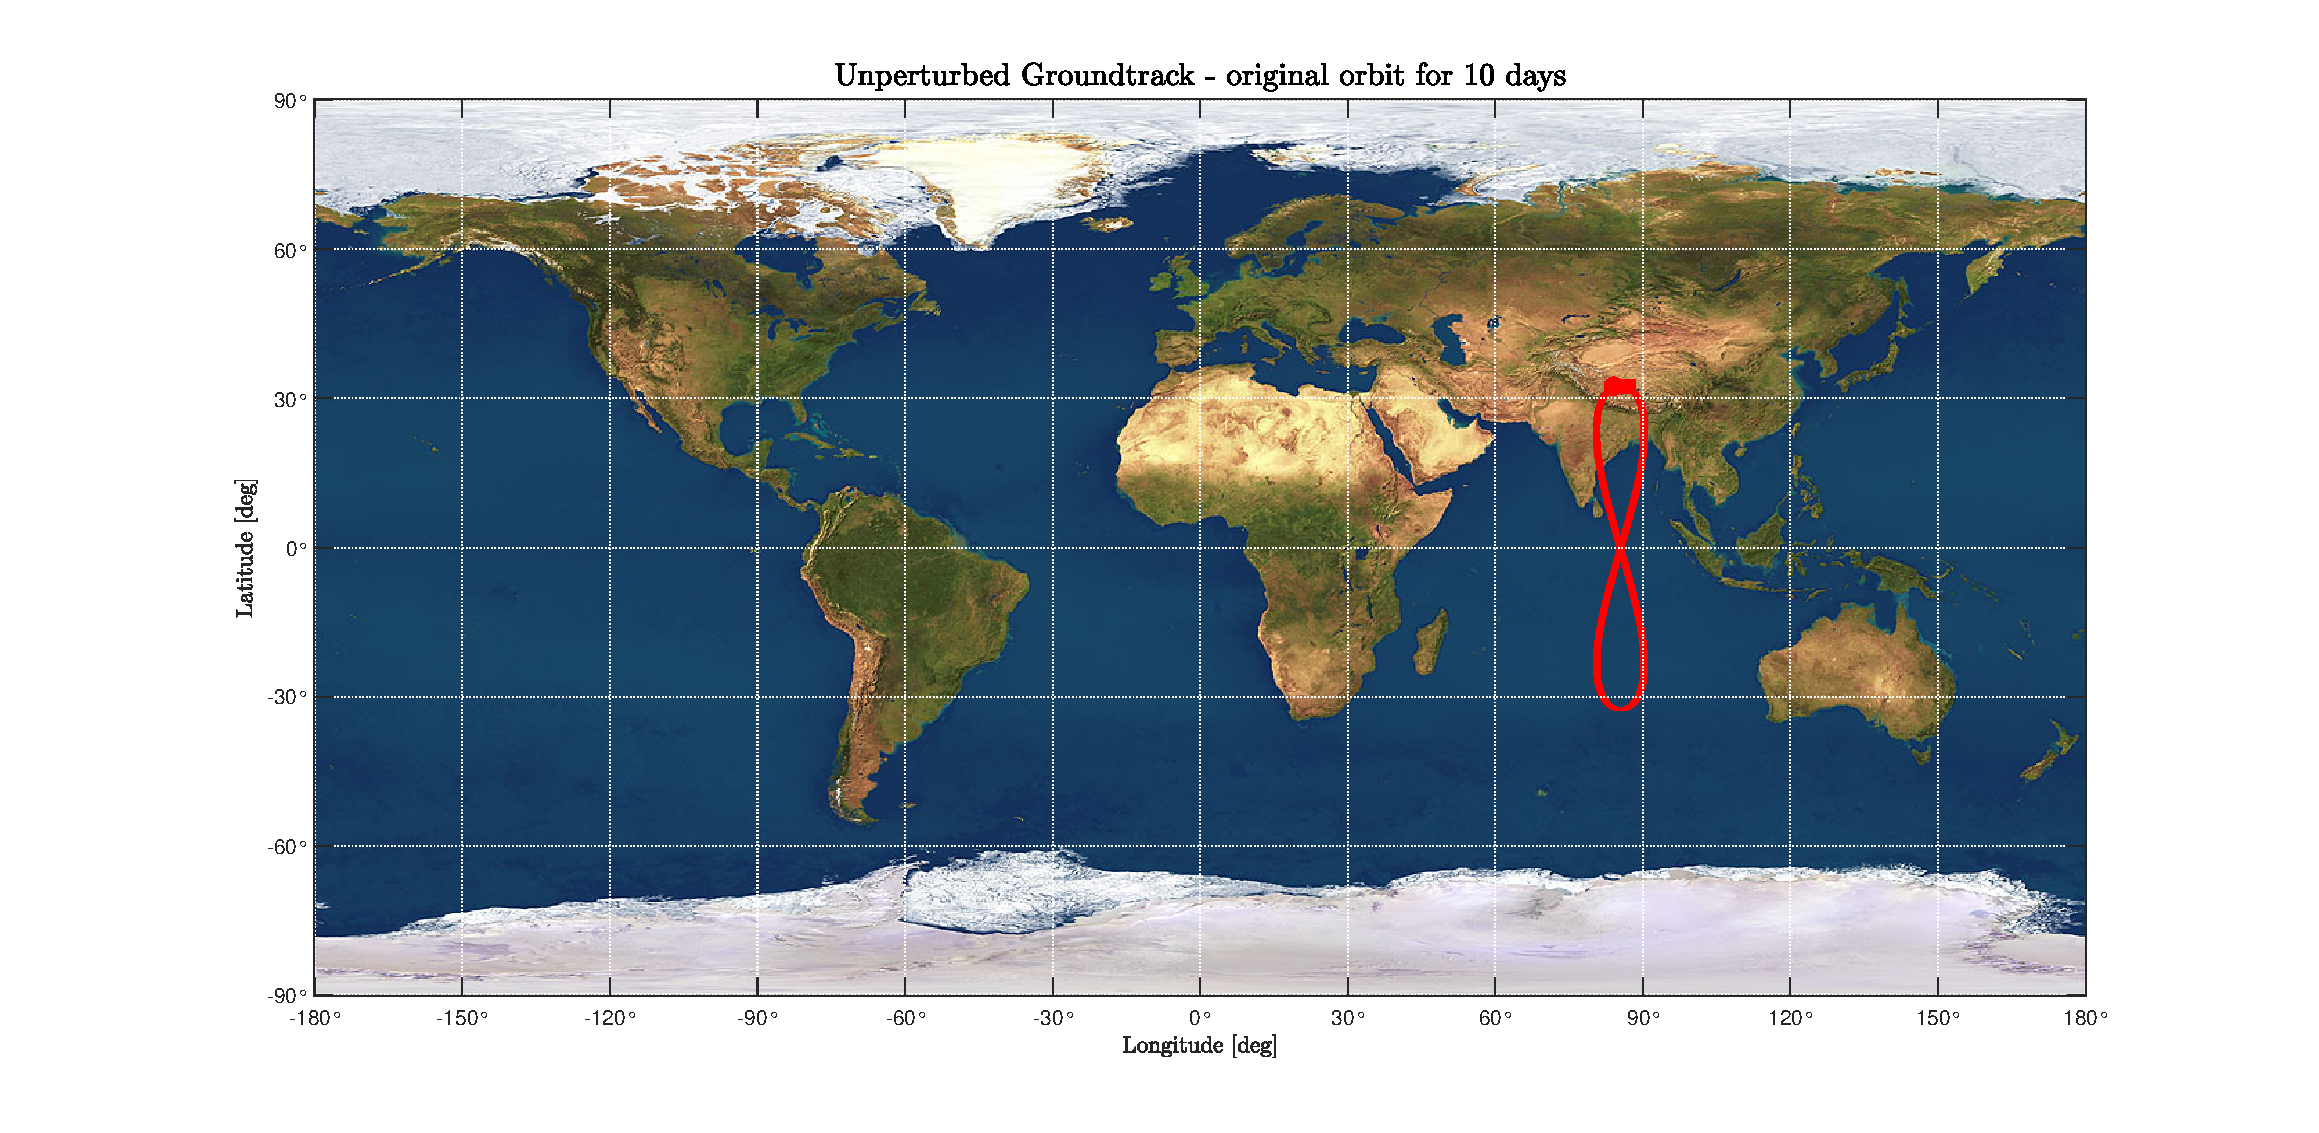
\includegraphics[width=\textwidth]{ug10d.eps}
		\caption{}
		\label{fig:1c}
	\end{subfigure}
	\hfill
	\begin{subfigure}[b]{0.45\textwidth}
		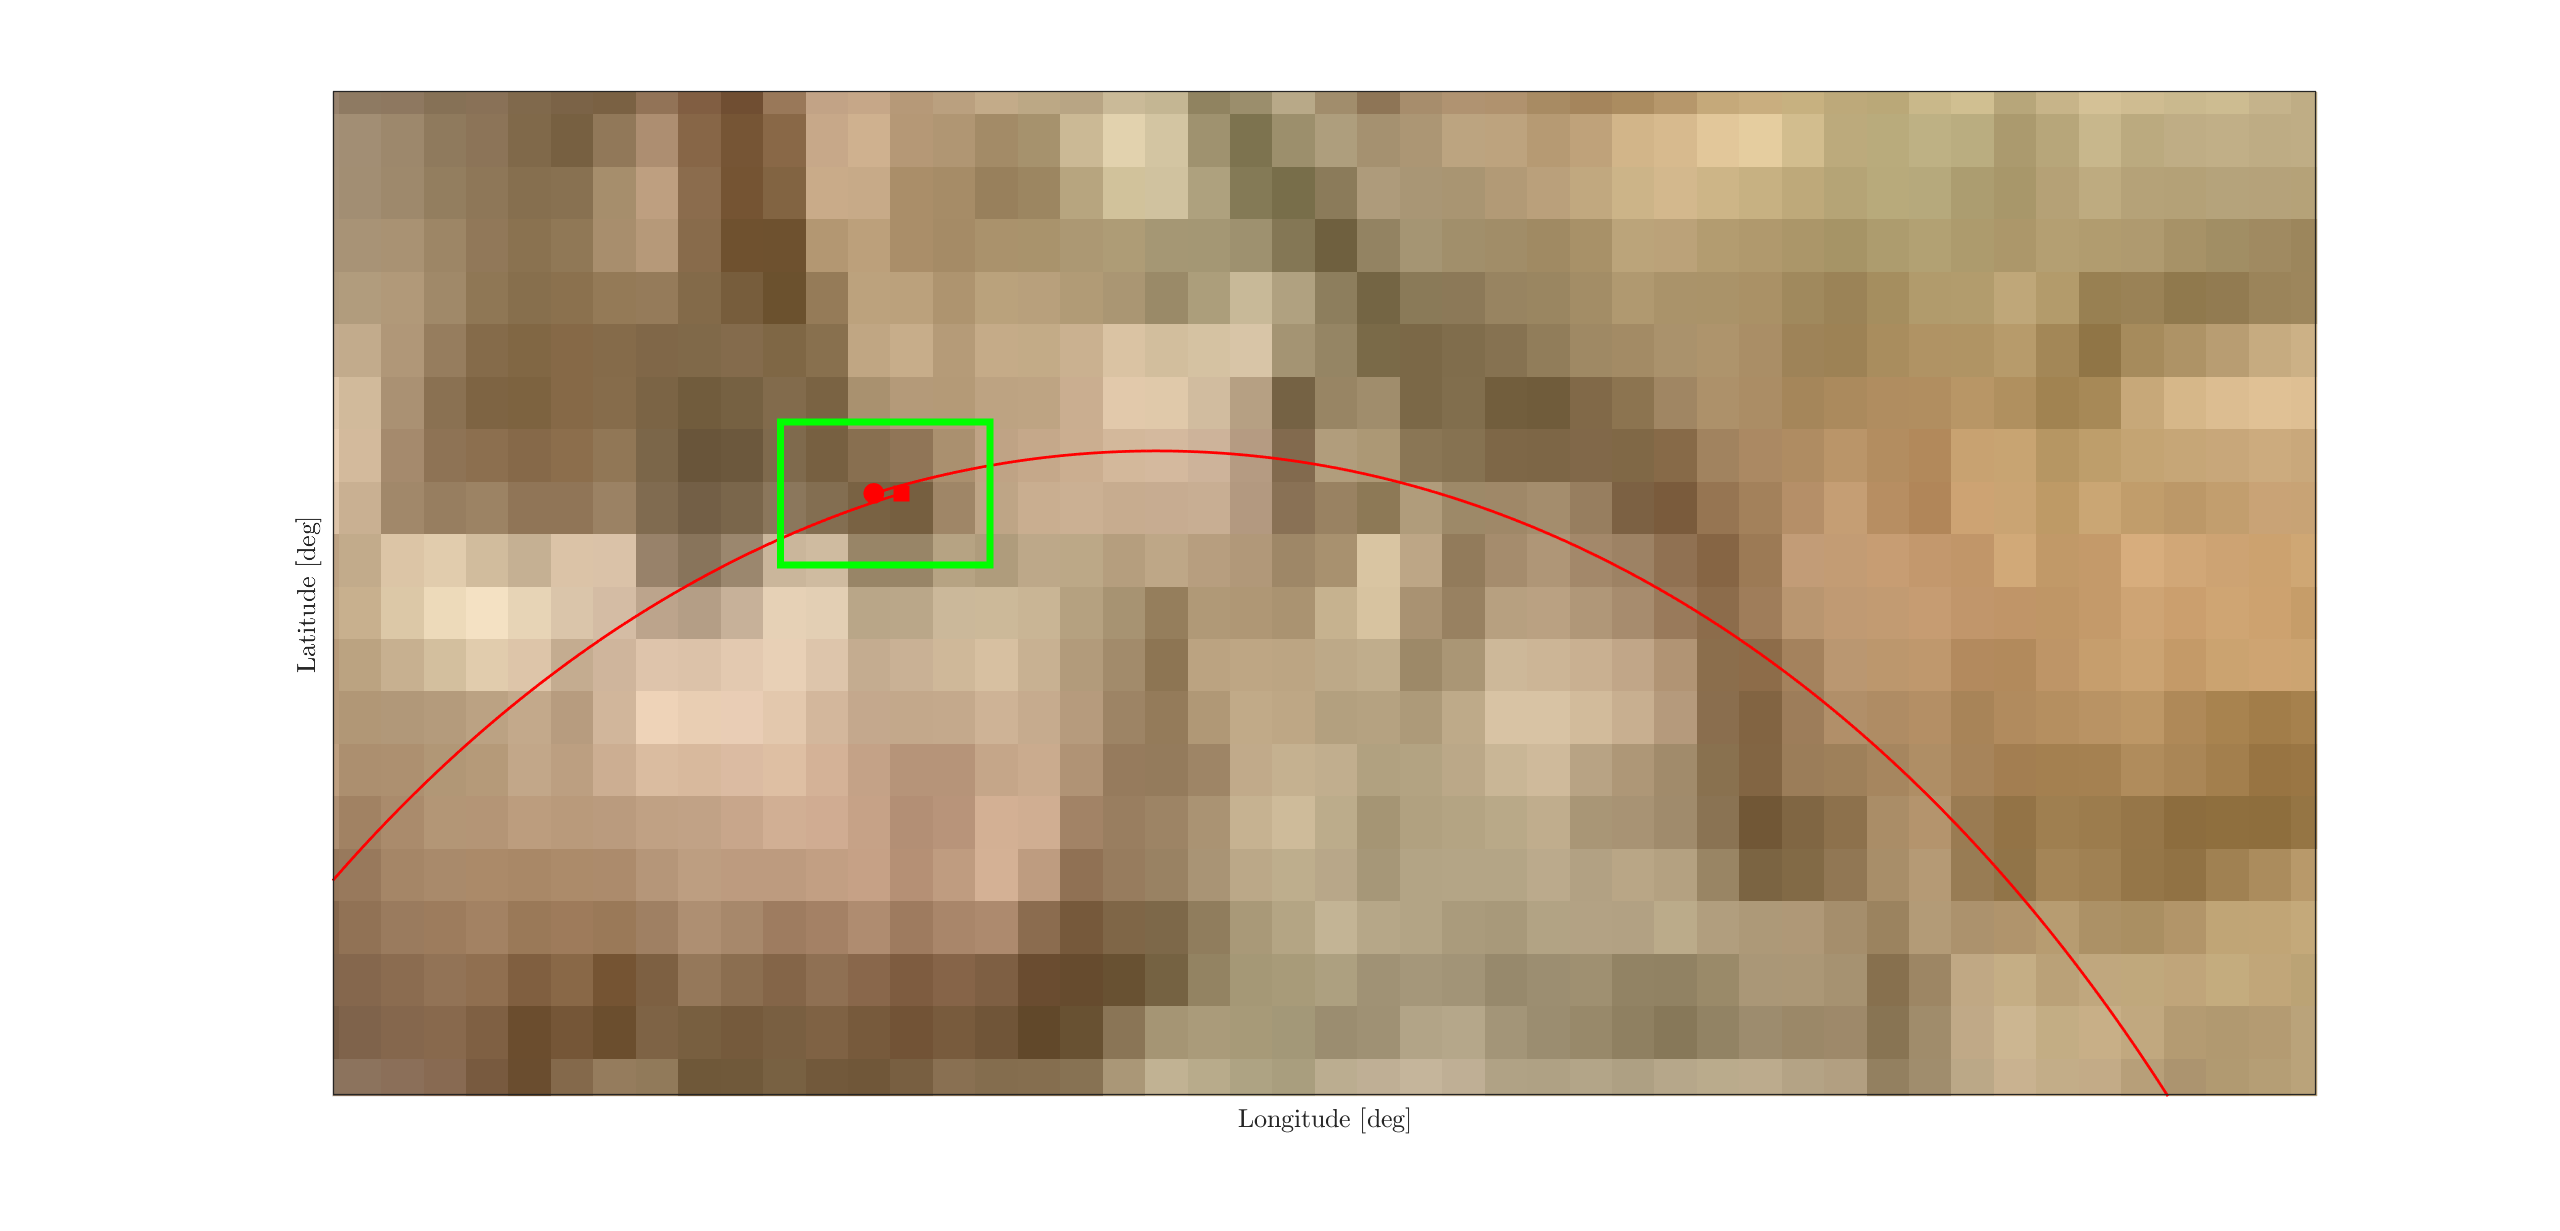
\includegraphics[width=\textwidth]{ugstartend.png}
		\caption{}
		\label{fig:1d}
	\end{subfigure}
	\caption{Ground track of the unperturbed nominal orbit during: (a) 1 orbit; (b) 1 day; (c) 10 days. Ground track path (\reddashedline), Starting point (\textcolor{red}{$\bullet$}), Ending point (\textcolor{red}{$\blacksquare$})
	}
\end{figure}


The groundtrack of this satellite has formed an “8” shape, a phenomenon known as the figure-eight groundtrack. At geosynchronous altitude, the location after one revolution is the same, and for geostationary  orbits, the satellite always appears to be stationary over one location. The figure “8” occurs because the satellites relative velocity is less and greater, than locations on the Earth as it travels from the ascending node. 


%cite: Vallado, Fundamentals of Astrodynamics, 2013

\subsubsection{Repeating Groundtrack}


For establishing a good communication with the network of ground stations of PoliMi Space Agency, a repeating ground track with a ratio of 1:1 (for each orbit of the spacecraft, Earth has performed 1 revolution) is maintained. Therefore, the period of the repeating ground track orbit is computed. For an unperturbed orbit, the period is only a function of the semi-major axis and can be calculated to get the desired repeating ground track. Both equations are listed below. By extension, the other orbital parameters are kept the same as the nominal orbit. 

	
\begin{equation*}
	T_{\text{repeating}} = \frac{1}{1} T_{\text{Earth}}
\end{equation*}

\begin{equation*}
	T = 2\pi \sqrt{\frac{a^3}{\mu}} \rightarrow a_{\text{repeating}} = \SI{42166}{\kilo\meter}
\end{equation*} 

\begin{figure}[H]
	\centering
	\begin{subfigure}[b]{0.45\textwidth}
		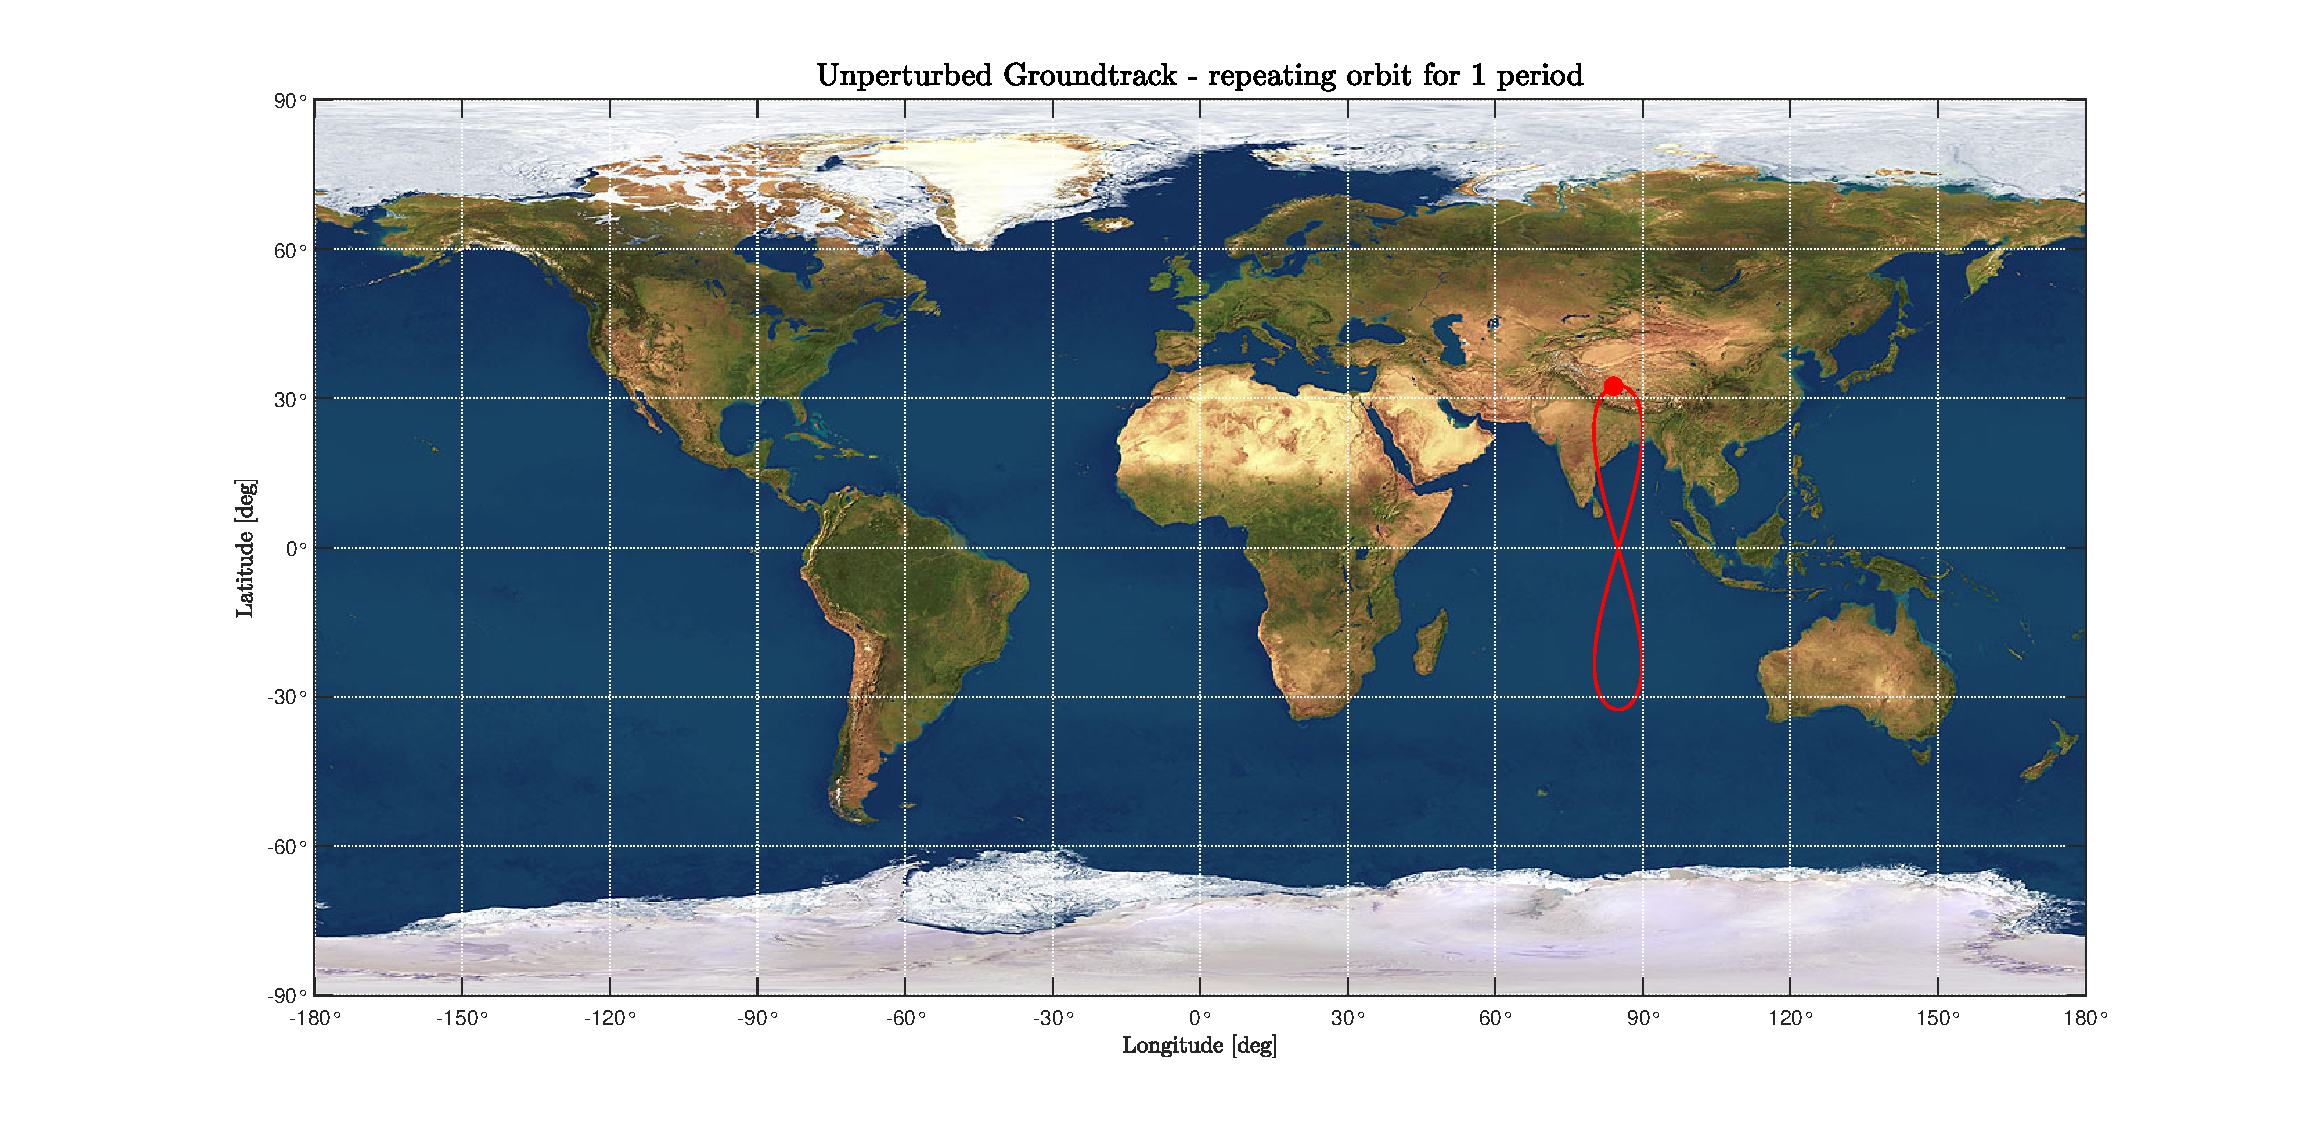
\includegraphics[width=\textwidth]{ugro1orb.eps}
		\caption{}
		\label{fig:1a}
	\end{subfigure}
	\hfill
	\begin{subfigure}[b]{0.45\textwidth}
		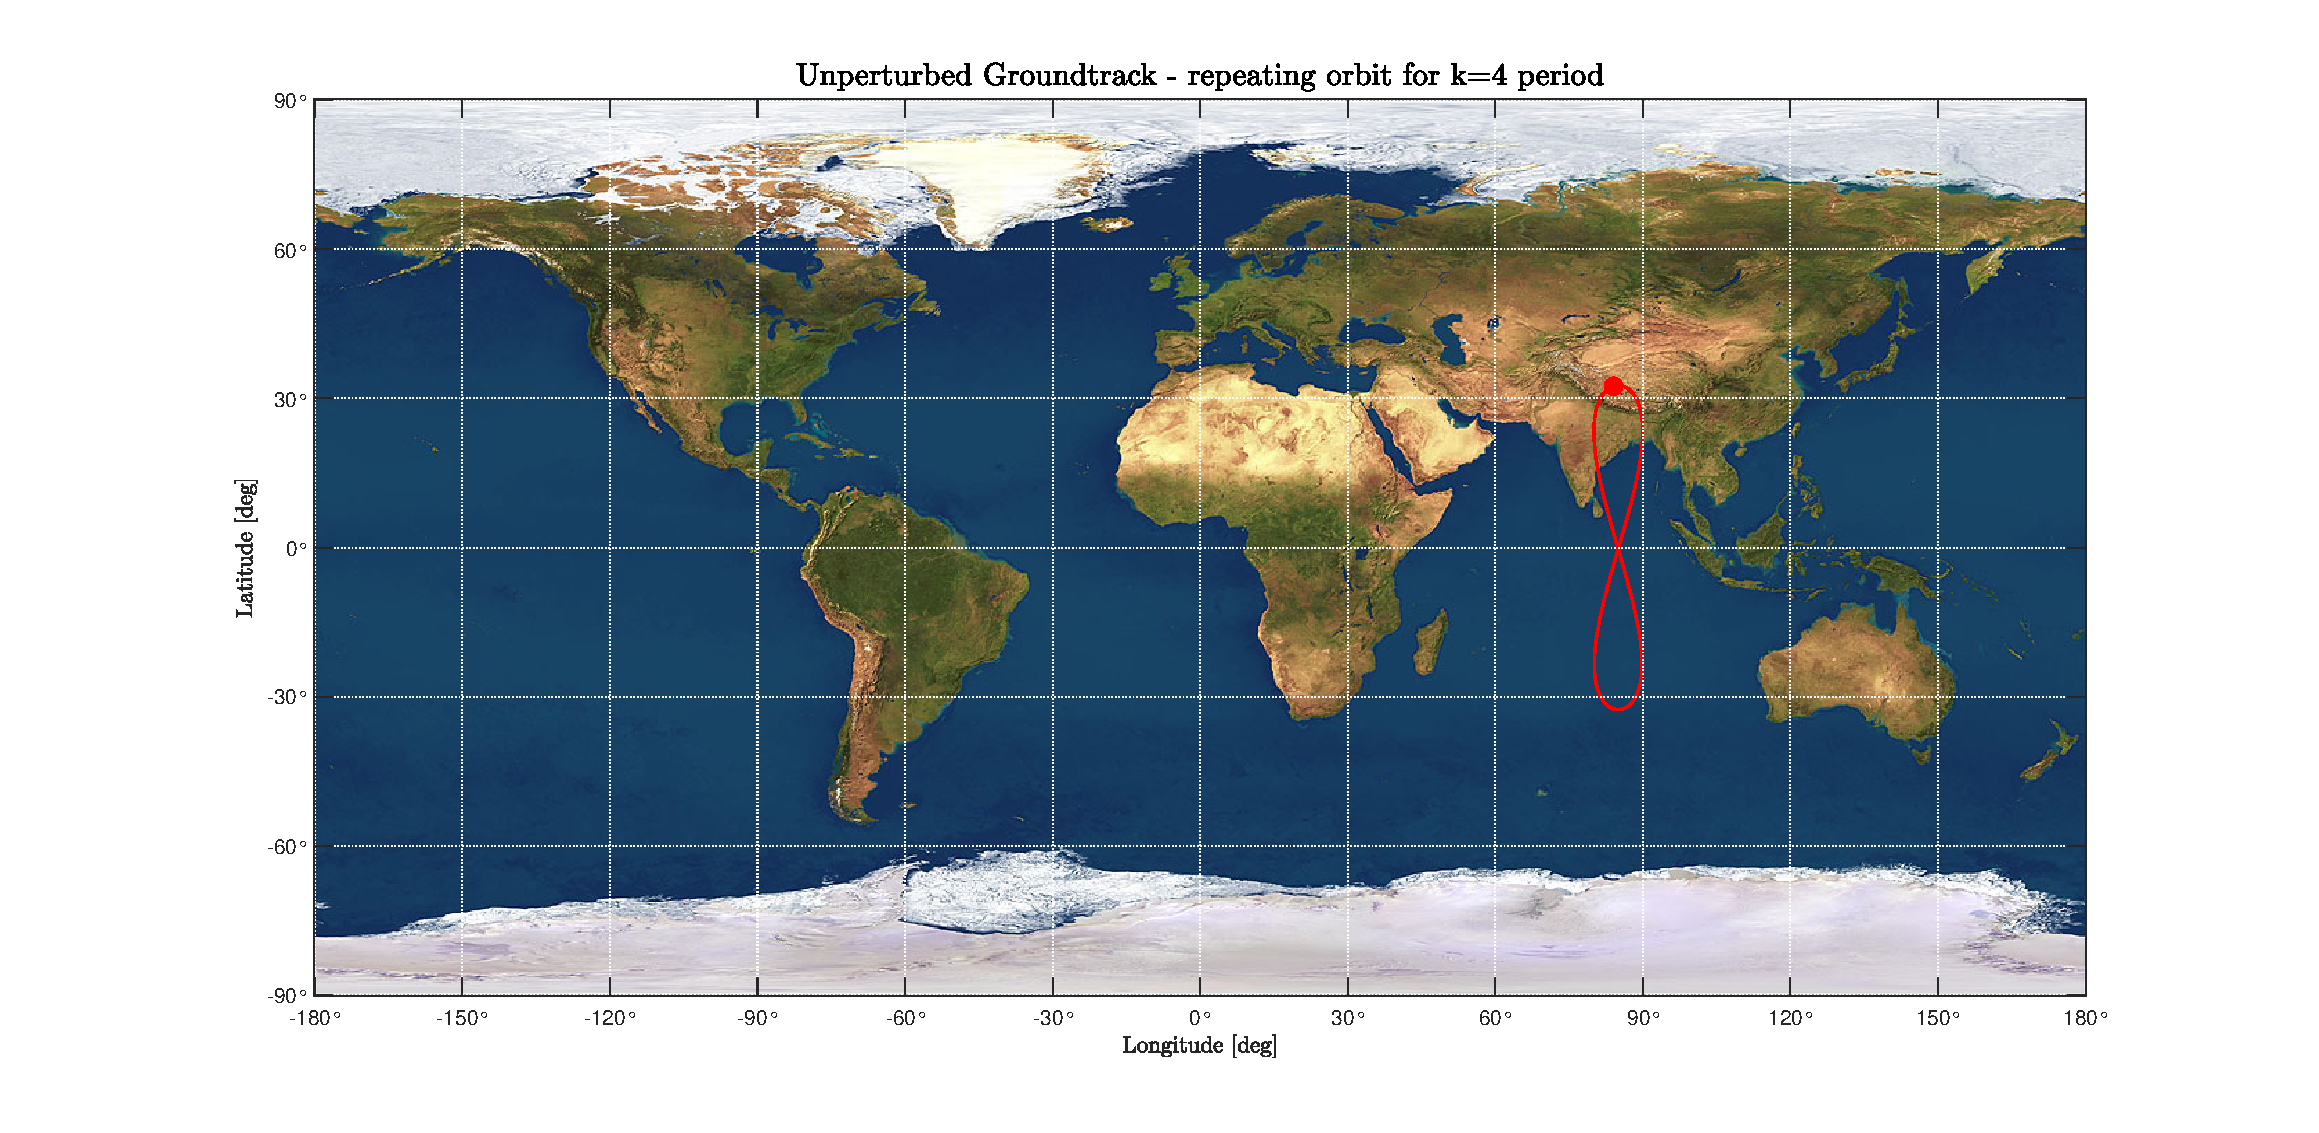
\includegraphics[width=\textwidth]{ugro4orb.eps}
		\caption{}
		\label{fig:1b}
	\end{subfigure}
	
	\caption{Ground track of the unperturbed repeating orbit during: (a) 1 orbit; (b) 4·k=4 orbits. Ground track path (\reddashedline), Starting point (\textcolor{red}{$\bullet$}), Ending point (\textcolor{red}{$\blacksquare$})
	}
\end{figure}

\subsection{Perturbed Groundtrack}
\subsubsection{Assigned Perturbations}

This project has been assigned with two perturbations: \( J_2 \) effect and Moon perturbation. \( J_2 \) effect consists of a perturbing potential on top of the central gravity field of the Earth. In order to model it, a zonal harmonic potential is used, function of the geocentric distance \( r \) and of the coelevation \( \phi \).

\begin{equation*}
	R(r, \phi) = \frac{\mu}{r} \left( -1 + \sum_{n=2}^{\infty} \left( \frac{R_E}{r} \right)^n J_n P_n(\cos\phi) \right)
\end{equation*}

Here, \( J_2 \) term is considered for modelling which is correlated to Earth oblateness. The perturbing acceleration due to \( J_2 \) effect is given as:

\begin{equation*}
	\mathbf{a}_{J_2} = \frac{3}{2} \frac{J_2 \mu R_E^2}{r^4} \left[ \left( \frac{x}{r} \left( \frac{5z^2}{r^2} - 1 \right) \right) \mathbf{i} + \left( \frac{y}{r} \left( \frac{5z^2}{r^2} - 1 \right) \right) \mathbf{j} + \left( \frac{z}{r} \left( \frac{5z^2}{r^2} - 3 \right) \right) \mathbf{k} \right]
\end{equation*}
%citation: Vallado, Curtis
Perturbation due to the moon acting on the orbit is modelled through a two body problem scenario taking into account the force of the moon as a perturbing acceleration. This acceleration is computed from:
\begin{equation*}
	\label{eq:moon_perturbation}
	\mathbf{a}_{\text{Moon}} = \mu_{\text{Moon}}
	\left( \frac{\mathbf{r}_{m/s}}{r_{m/s}^3} - \frac{\mathbf{r}_m}{r_m^3} \right)
\end{equation*}
where \( \mathbf{r}_{m/s} \) is the vector that goes from the S/C to the moon and \( \mathbf{r}_m \) is the vector that goes from Earth to Moon.\\ 

Possible perturbations are charted in \ref{fig:orbit perturbations}. It is observed that the \( J_2 \) effect (\( C_{2,0} \) in figure) and moon perturbation are one of the primary sources of orbital perturbation. Hence, our models and altitude choice are consistent.   

\begin{figure}[H]
	\centering
	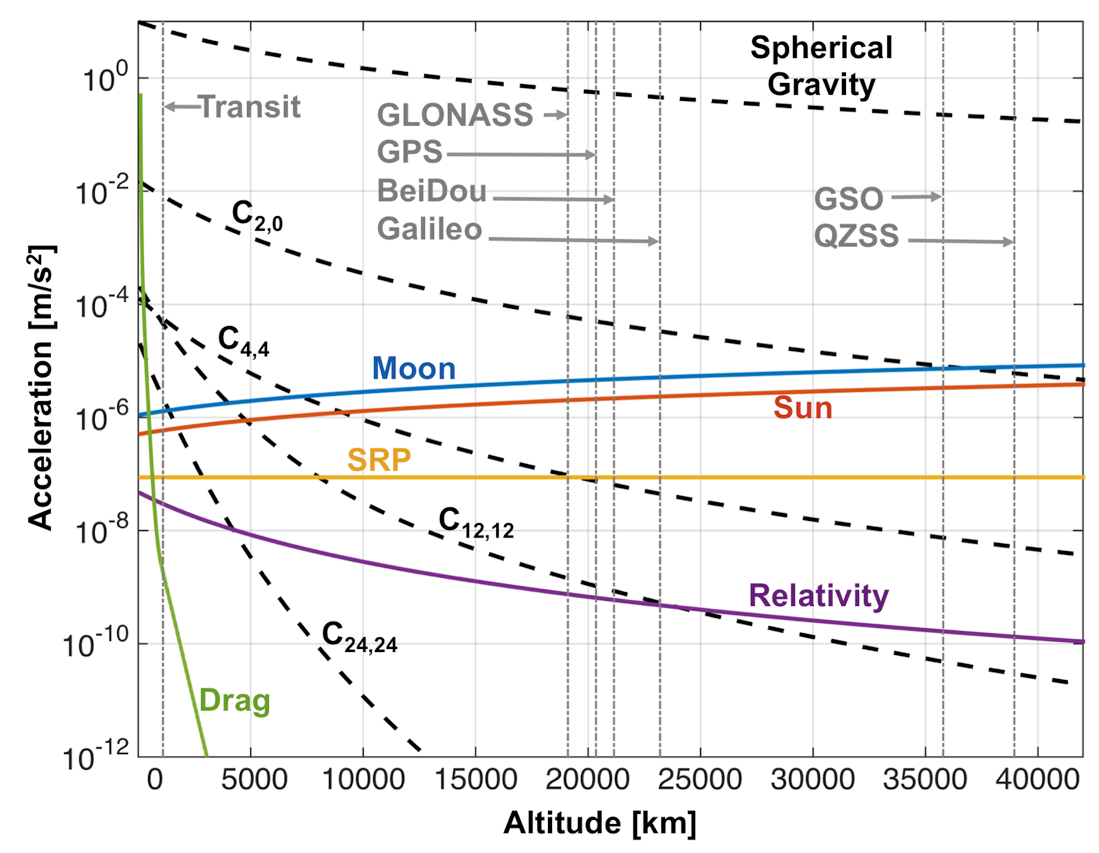
\includegraphics[width=0.5\textwidth]{Perturbation chart.png}
	\caption{Orbit Perturbations.}
	\label{fig:orbit perturbations}
\end{figure}

%Citation: T. G. R. Reid. ORBITAL DIVERSITY FOR GLOBAL NAVIGATION SATELLITE SYSTEMS. Stanford University, 2017.

\subsubsection{Nominal and Repeating Groundtrack}

\begin{figure}[H]
	\centering
	\begin{subfigure}[b]{0.45\textwidth}
		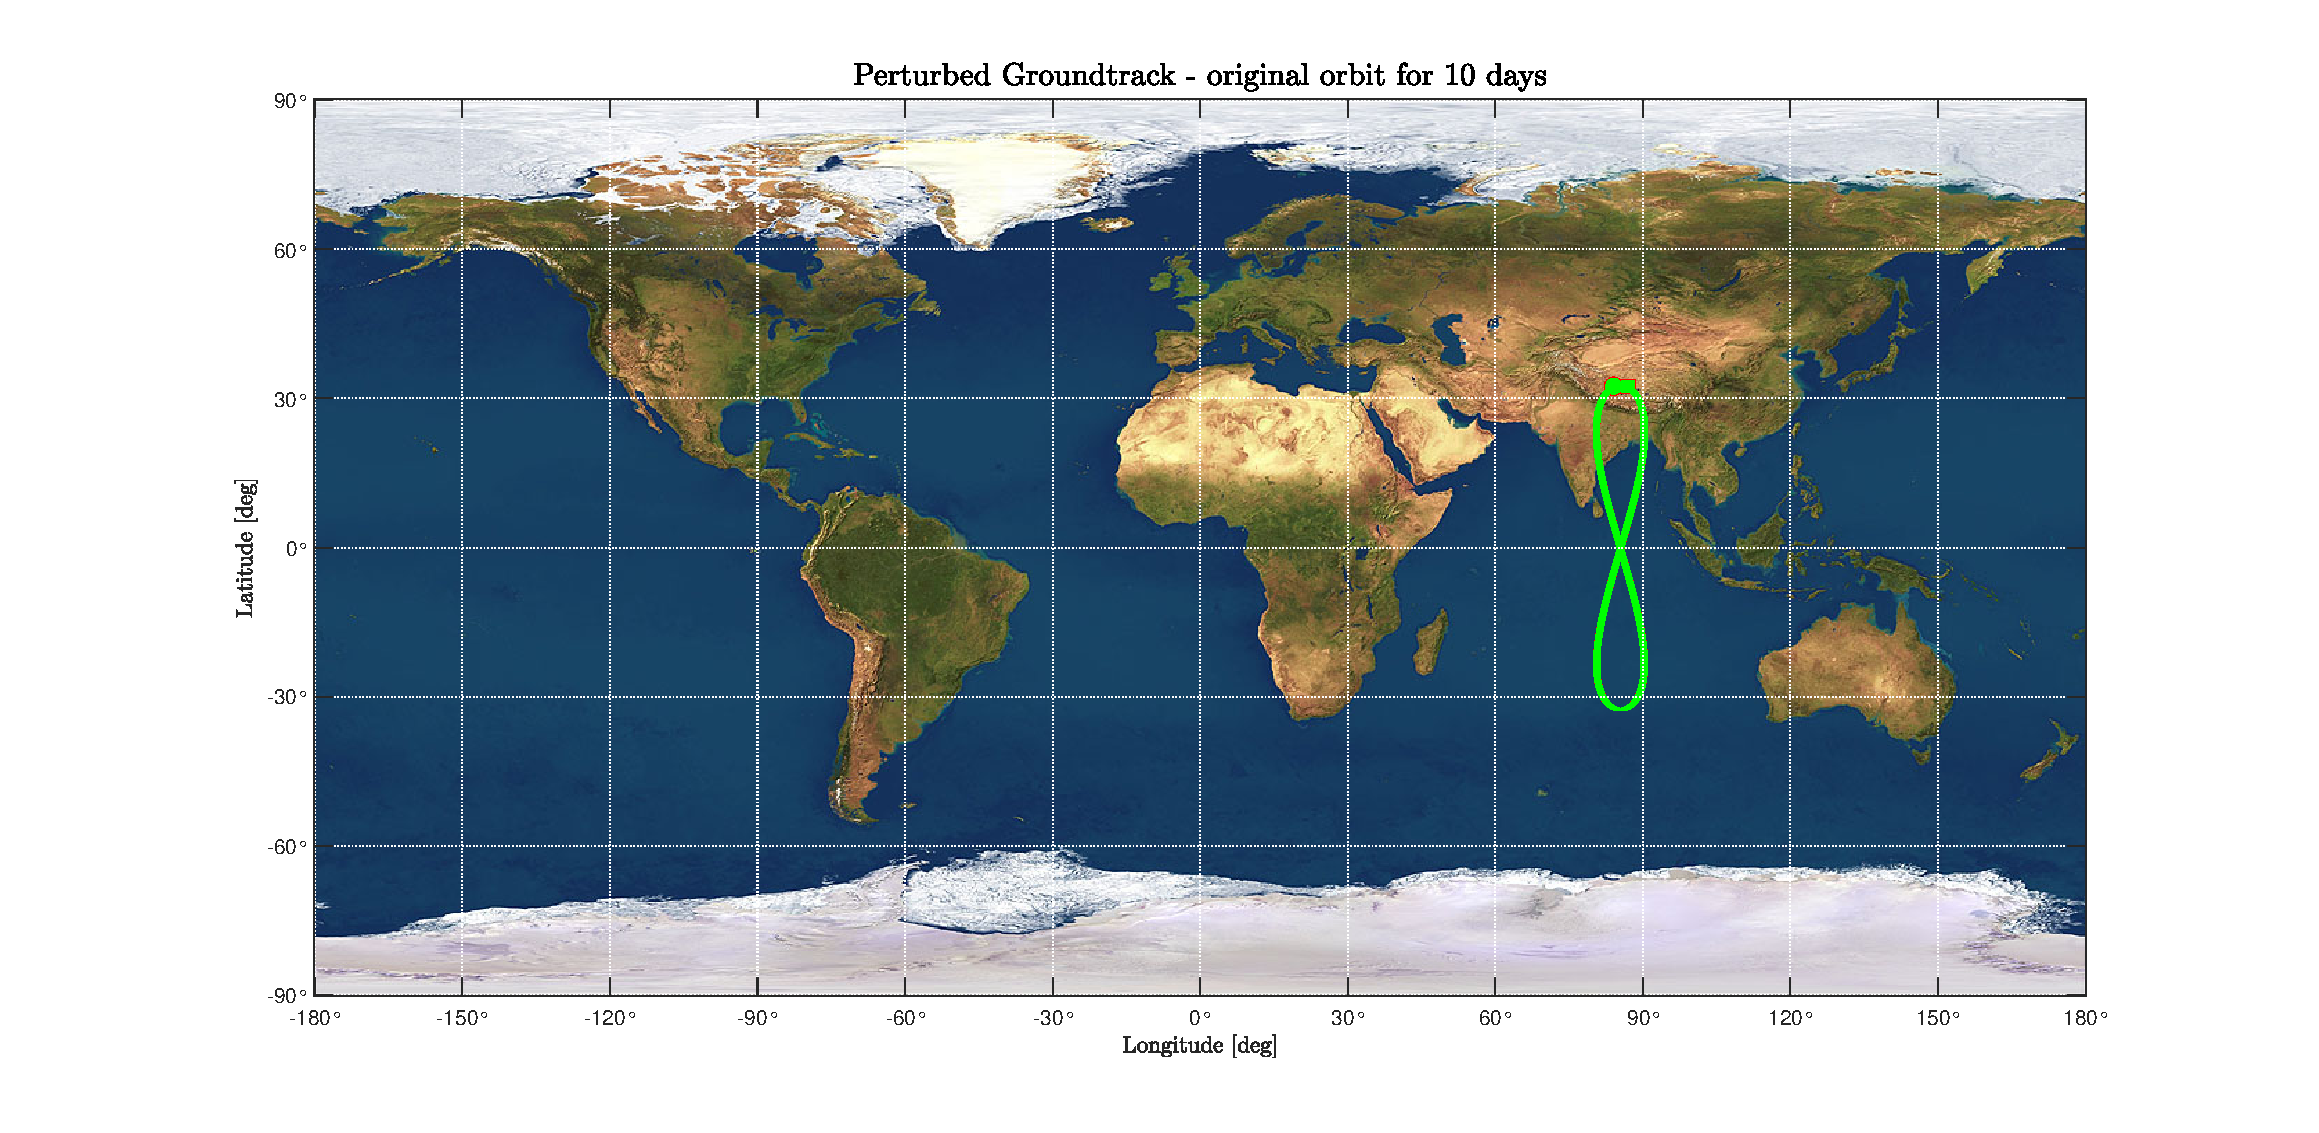
\includegraphics[width=\textwidth]{pg10d.eps}
		\caption{}
		\label{fig:5a}
	\end{subfigure}
	\hfill
	\begin{subfigure}[b]{0.45\textwidth}
		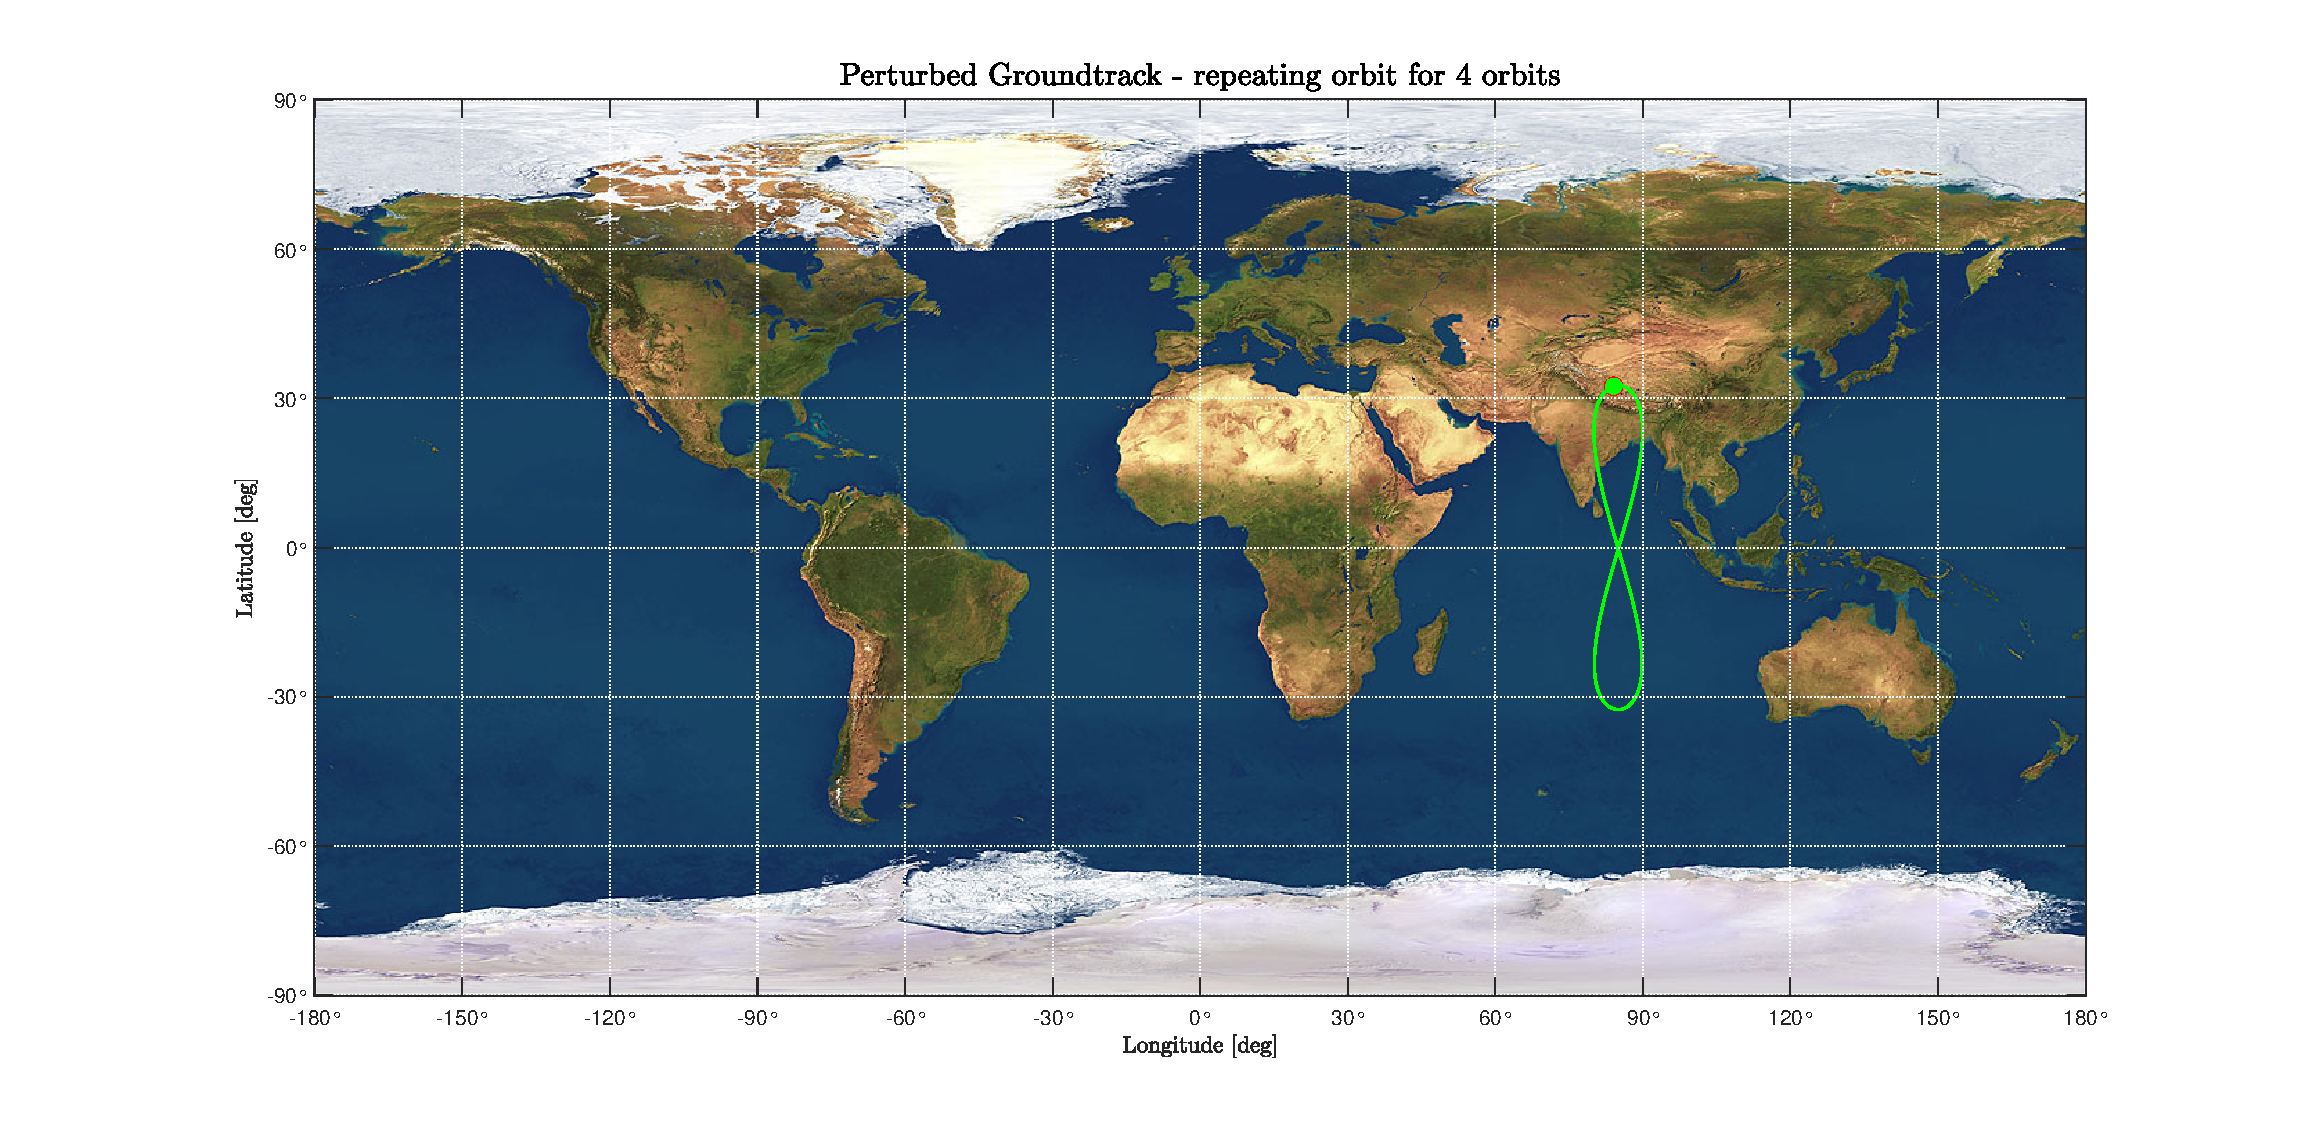
\includegraphics[width=\textwidth]{pgro4orb.eps}
		\caption{}
		\label{fig:5b}
	\end{subfigure}
	
	\vspace{1cm} 
	\begin{subfigure}[b]{0.45\textwidth}
		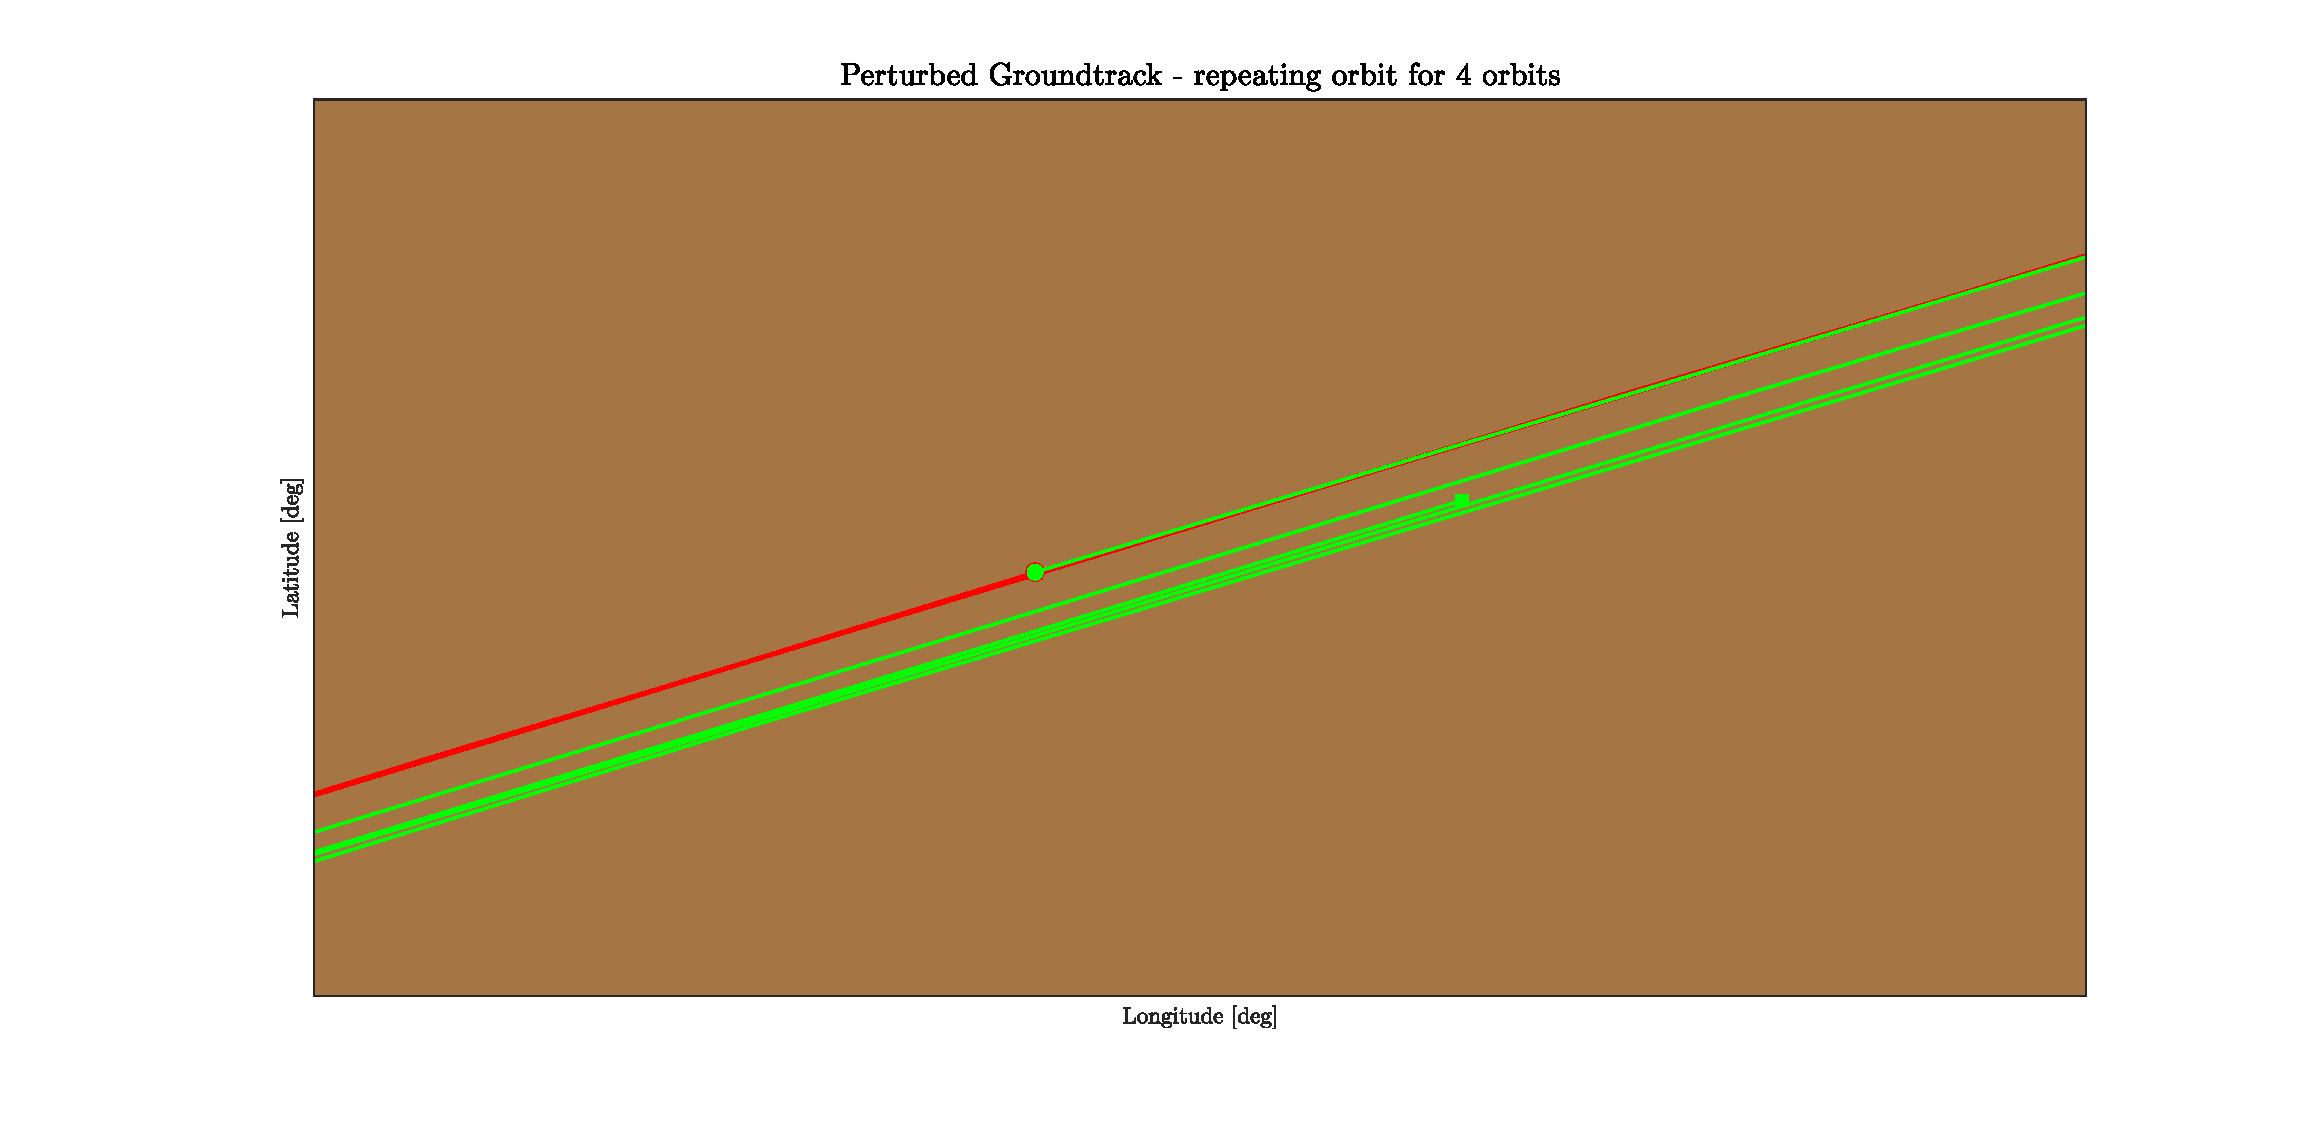
\includegraphics[width=\textwidth]{zoompgro4orb.eps}
		\caption{}
		\label{fig:5c}
	\end{subfigure}
	
	\caption{Ground track of the perturbed orbits: (a) Nominal orbit during 10 days; (b) Repeating orbit during 4 orbits; (c) Perturbation effect for repeating orbit. Ground track of unperturbed (\reddashedline), Starting point (\textcolor{red}{$\bullet$}), Ending point (\textcolor{red}{$\blacksquare$}); Ground track of perturbed (\greendashedline), Starting point (\textcolor{green}{$\bullet$}), Ending point (\textcolor{green}{$\blacksquare$}).
	}
\end{figure}

It is observed that the perturbations have a great impact on the ground track path of the satellite. Both the nominal and repeating orbits get out of phase with relation to the unperturbed case. From \ref{fig:5c}, the repeating ground track orbit proposed does not work in the presence of assigned perturbations. 

\section{Orbit Propagation}

Orbits were propagated using Cartesian coordinates (Newton’s equations of motion), or Keplerian elements (Gauss’ planetary equations). Gauss' equations are presented in the Radial-Transversal-Out-of-plane reference frame (RSW). All formulas can be found in ().\\ %{cite: Curtis}

\begin{align*}
	\frac{da}{dt} &= \frac{2a^2}{h} \left( e\sin f a_r + \frac{p}{r} a_s \right) \\[10pt]
	\frac{de}{dt} &= \frac{1}{h} \left( p\sin f a_r + \left( (p + r) \cos f + re \right) a_s \right) \\[10pt]
	\frac{di}{dt} &= \frac{r\cos (f + \omega)}{h} a_w \\[10pt]
	\frac{d\Omega}{dt} &= \frac{r\sin (f + \omega)}{h\sin i} a_w \\[10pt]
	\frac{d\omega}{dt} &= \frac{1}{he} \left( -p\cos f a_r + (p + r)\sin f a_s \right) - \frac{r\sin(f + \omega) \cos i}{h\sin i} a_w \\[10pt]
	\frac{df}{dt} &= \frac{h}{r^2} + \frac{1}{eh} \left( p\cos f a_r - (p + r)\sin f a_s \right)
\end{align*}
\\

For the moon perturbation, which cannot be directly expressed in RSW frame, it's possible to transform the perturbing accelerations from Cartesian to RSW. The three rotation matrices for this are shown below where a rotation of \(\Omega\) around the third axis of the inertial frame is performed, then a rotation of \(i\) around the first axis of the rotated frame, and finally a rotation of an angle \(\theta\ + \omega\) around the third axis of the last frame. 

\[
R_{\Omega} = \begin{bmatrix}
	\cos \Omega & \sin \Omega & 0 \\
	-\sin \Omega & \cos \Omega & 0 \\
	0 & 0 & 1
\end{bmatrix}, \quad
R_{i} = \begin{bmatrix}
	1 & 0 & 0 \\
	0 & \cos i & \sin i \\
	0 & -\sin i & \cos i
\end{bmatrix}, \quad
R_{\theta + \omega} = \begin{bmatrix}
	\cos (\theta + \omega) & \sin (\theta + \omega) & 0 \\
	-\sin (\theta + \omega) & \cos (\theta + \omega) & 0 \\
	0 & 0 & 1
\end{bmatrix}
\]

\subsection{History of the Keplerian Elements} 

The Keplerian elements were obtained through the integration of the equation of motion and of the Gauss planetary equations. The propagation time is taken as 10 years, so it's sufficient to see the perturbations properly developed for this project's case. The evolution of the data and of the relative error between both methods of integration are presented below:

\begin{figure}[H]
	\centering
	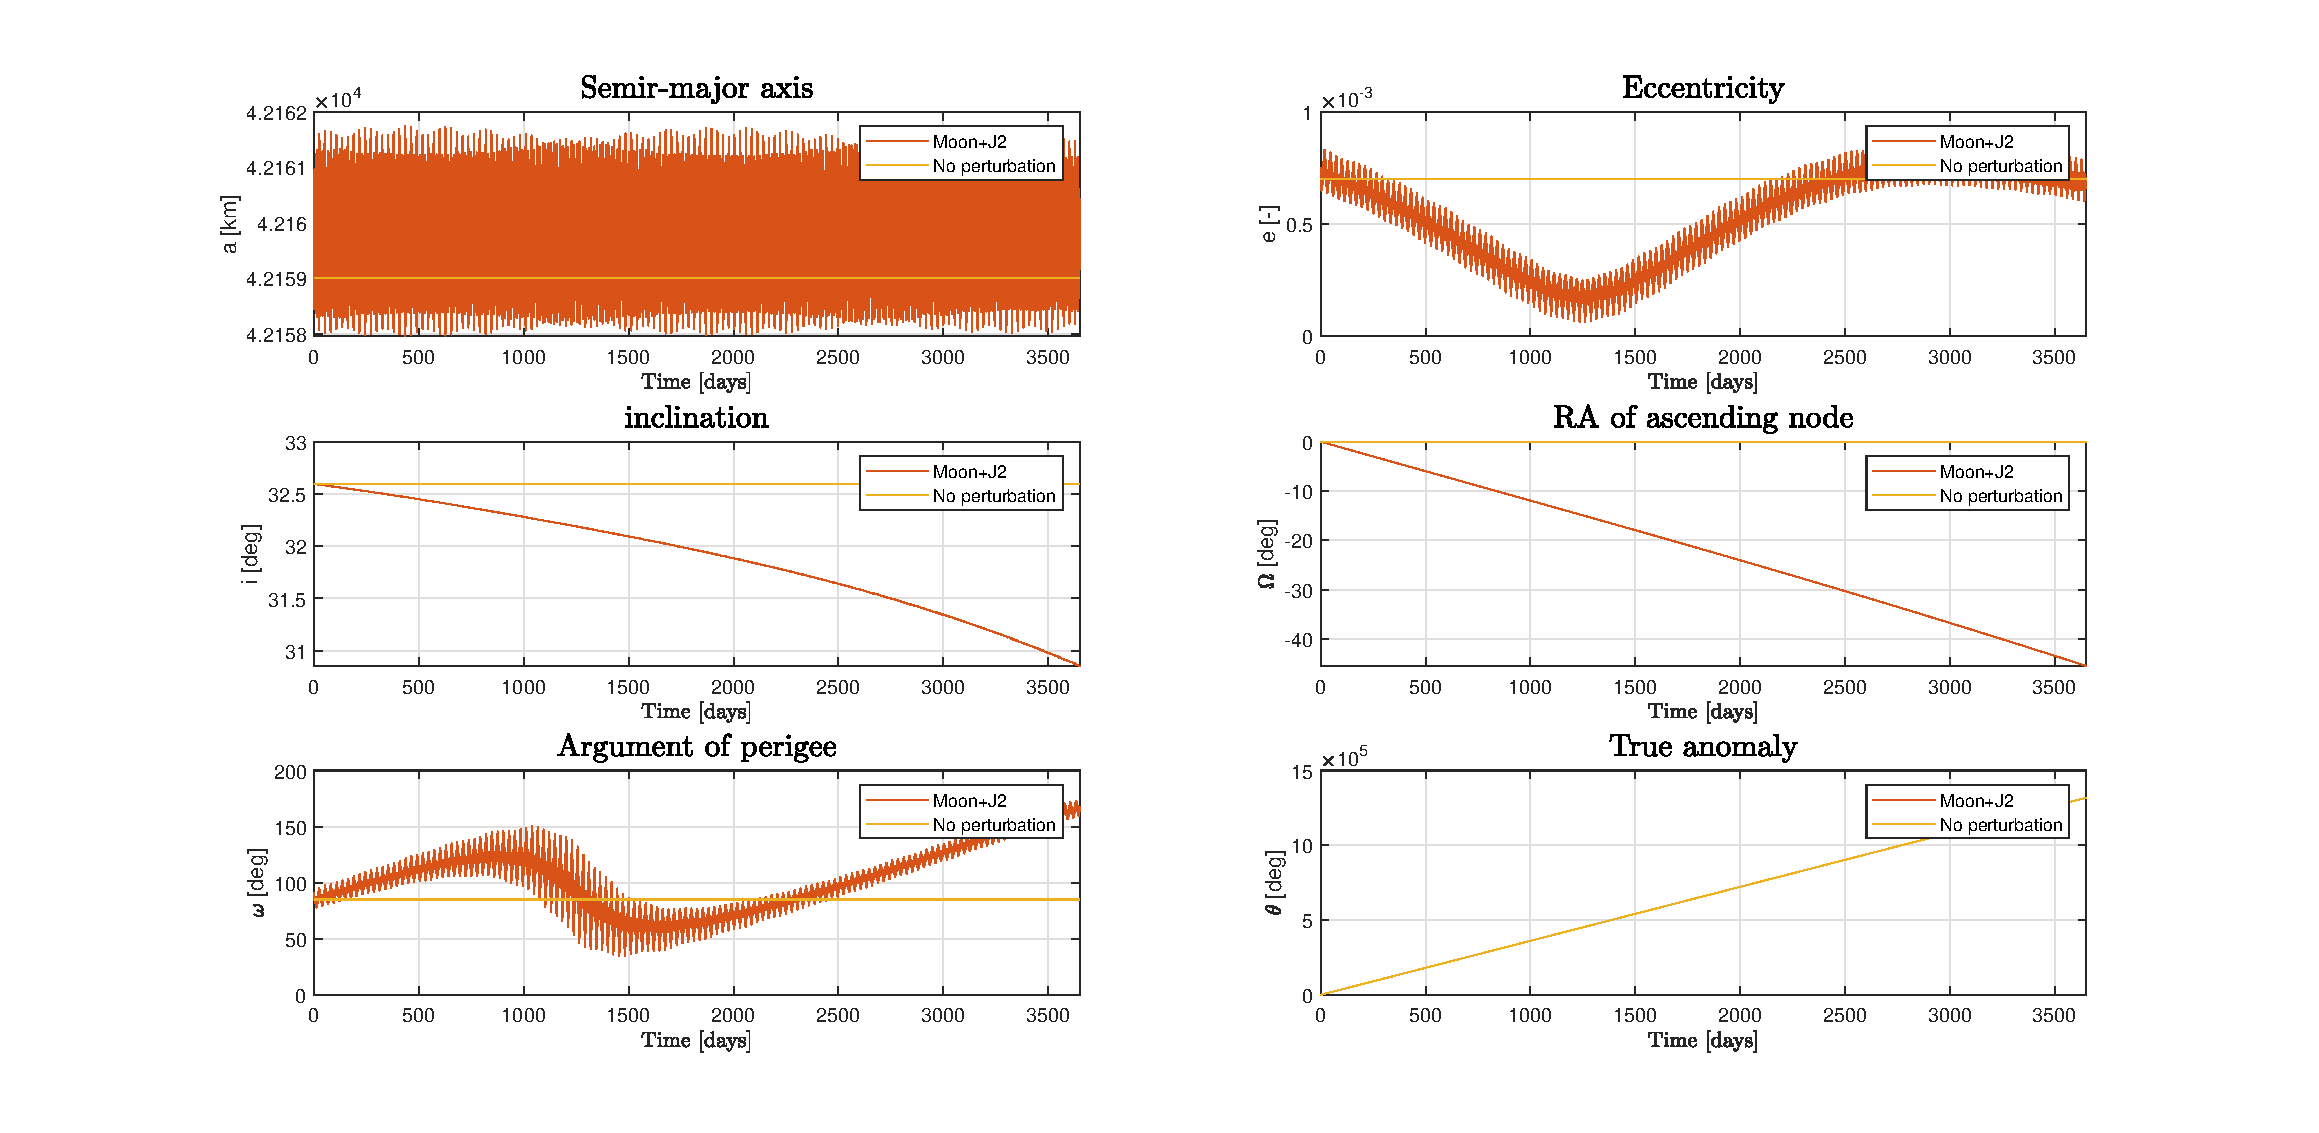
\includegraphics[width=1\textwidth]{orbitprop10yrs.eps}
	\caption{Evolution of the data.}
	\label{fig:orbitprop10yrs}
\end{figure}

\begin{figure}[H]
	\centering
	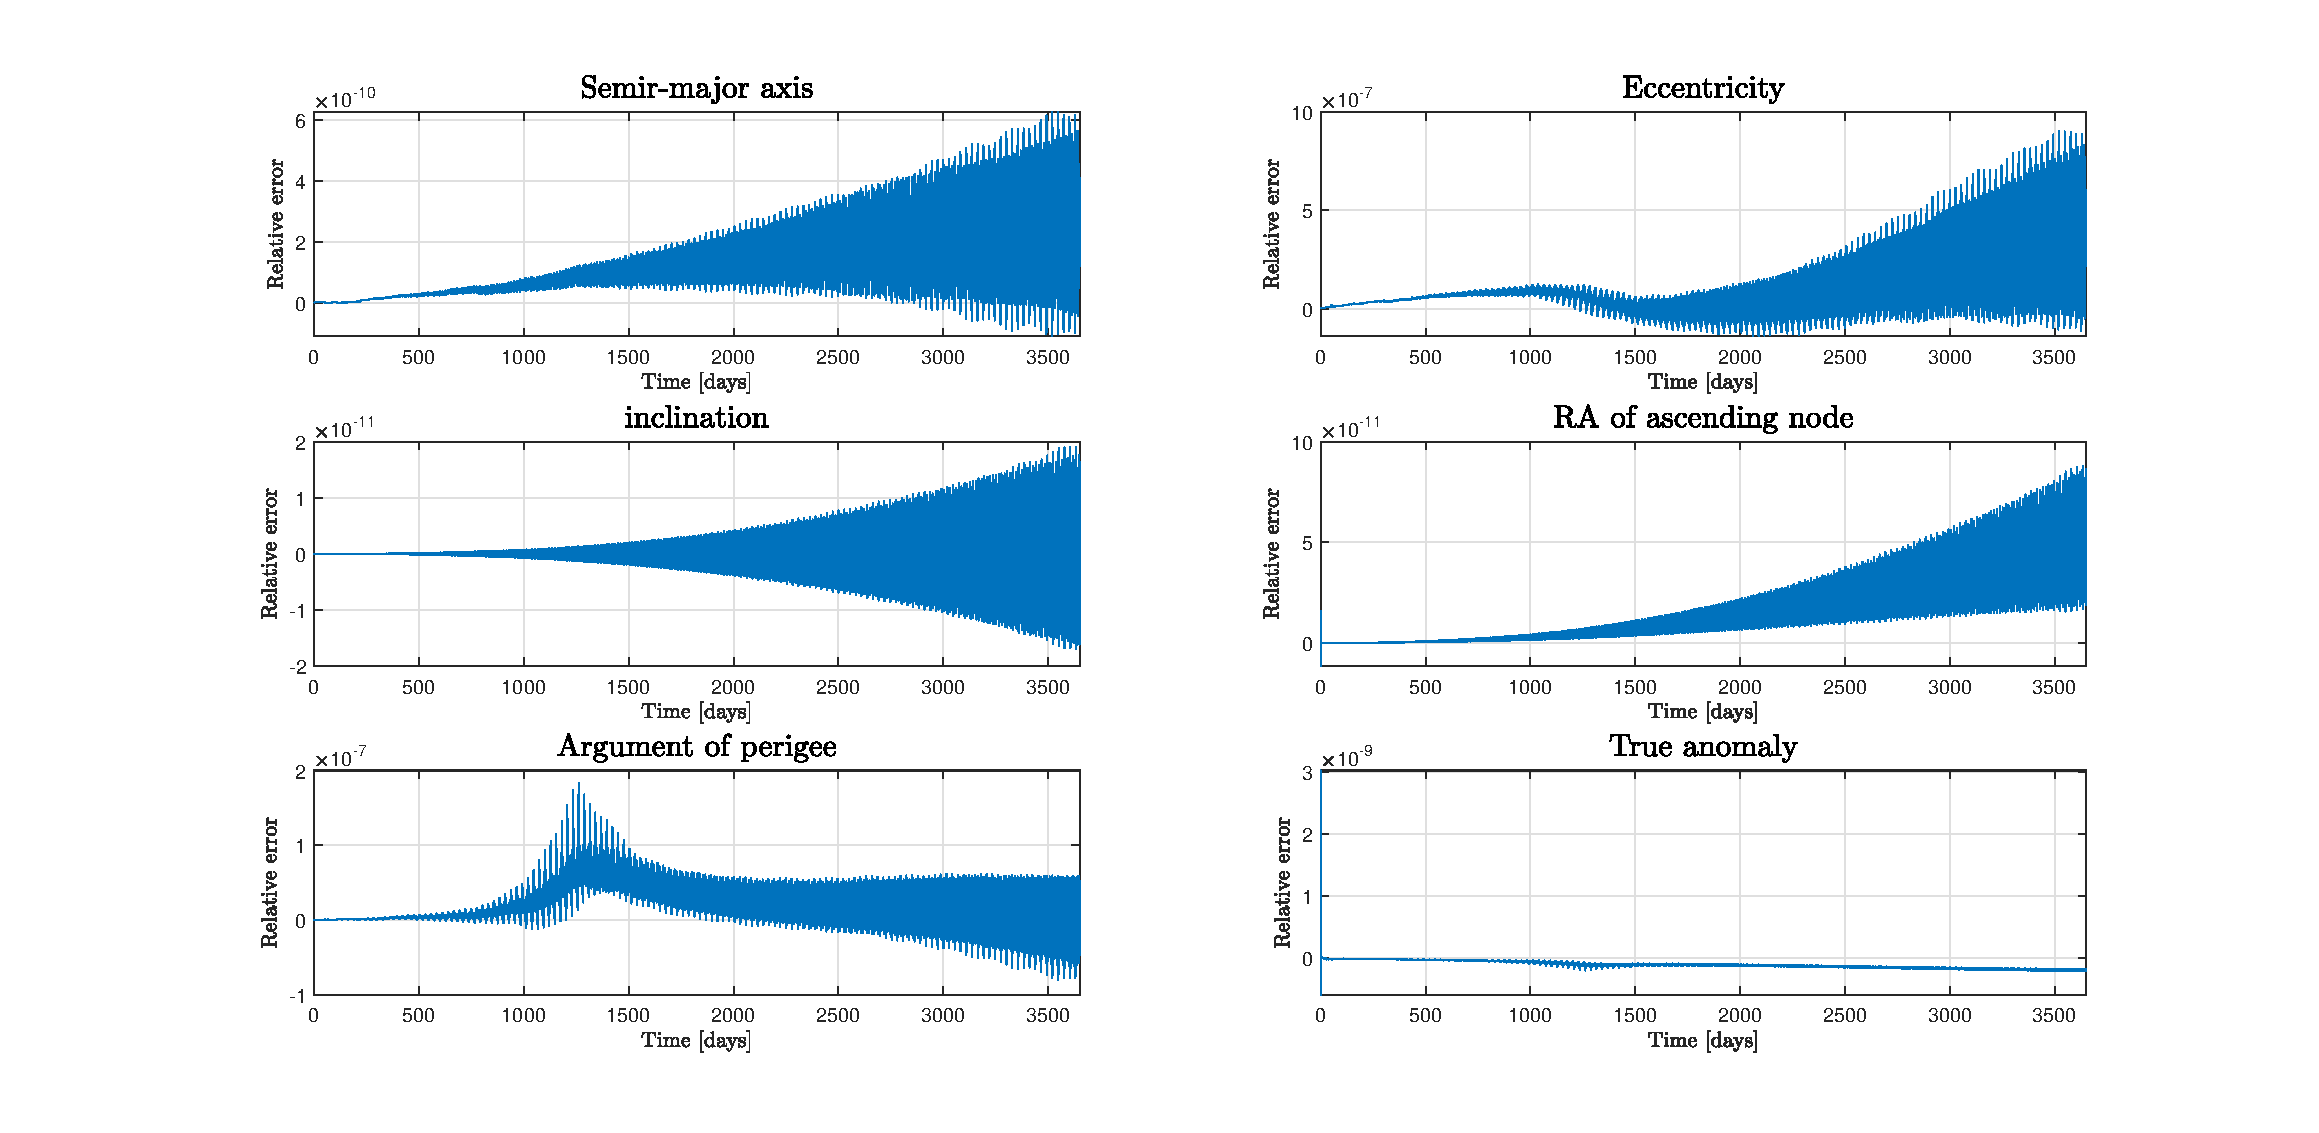
\includegraphics[width=1\textwidth]{relative_error10yrs.eps}
	\caption{Relative error between both methods of integration.}
	\label{fig:relative_error10yrs}
\end{figure}

It is possible to distinguish a long-periodic behaviour and a short-periodic behaviour by looking at the evolution of orbital elements. It is very clear for eccentricity \( e \), inclination \( i \), and also for argument of perigee \( \omega \) to a sufficient extent. Semi-major axis presents both short-periodic and long-periodic behaviour. As for the right ascension of ascending node \( \Omega \), and true anomaly \( f \), the short-periodic behaviour is less visible but still present. From the figure \ref{fig:relative_error10yrs} of relative error between Gauss’ resolution and Cartesian resolution, it can be observed that the two methods are equivalent if the precision of the two is compared.

\subsection{Representation of the Evolution of the Orbit} 

\begin{figure}[H]
	\centering
	\begin{subfigure}[b]{0.5\textwidth}
		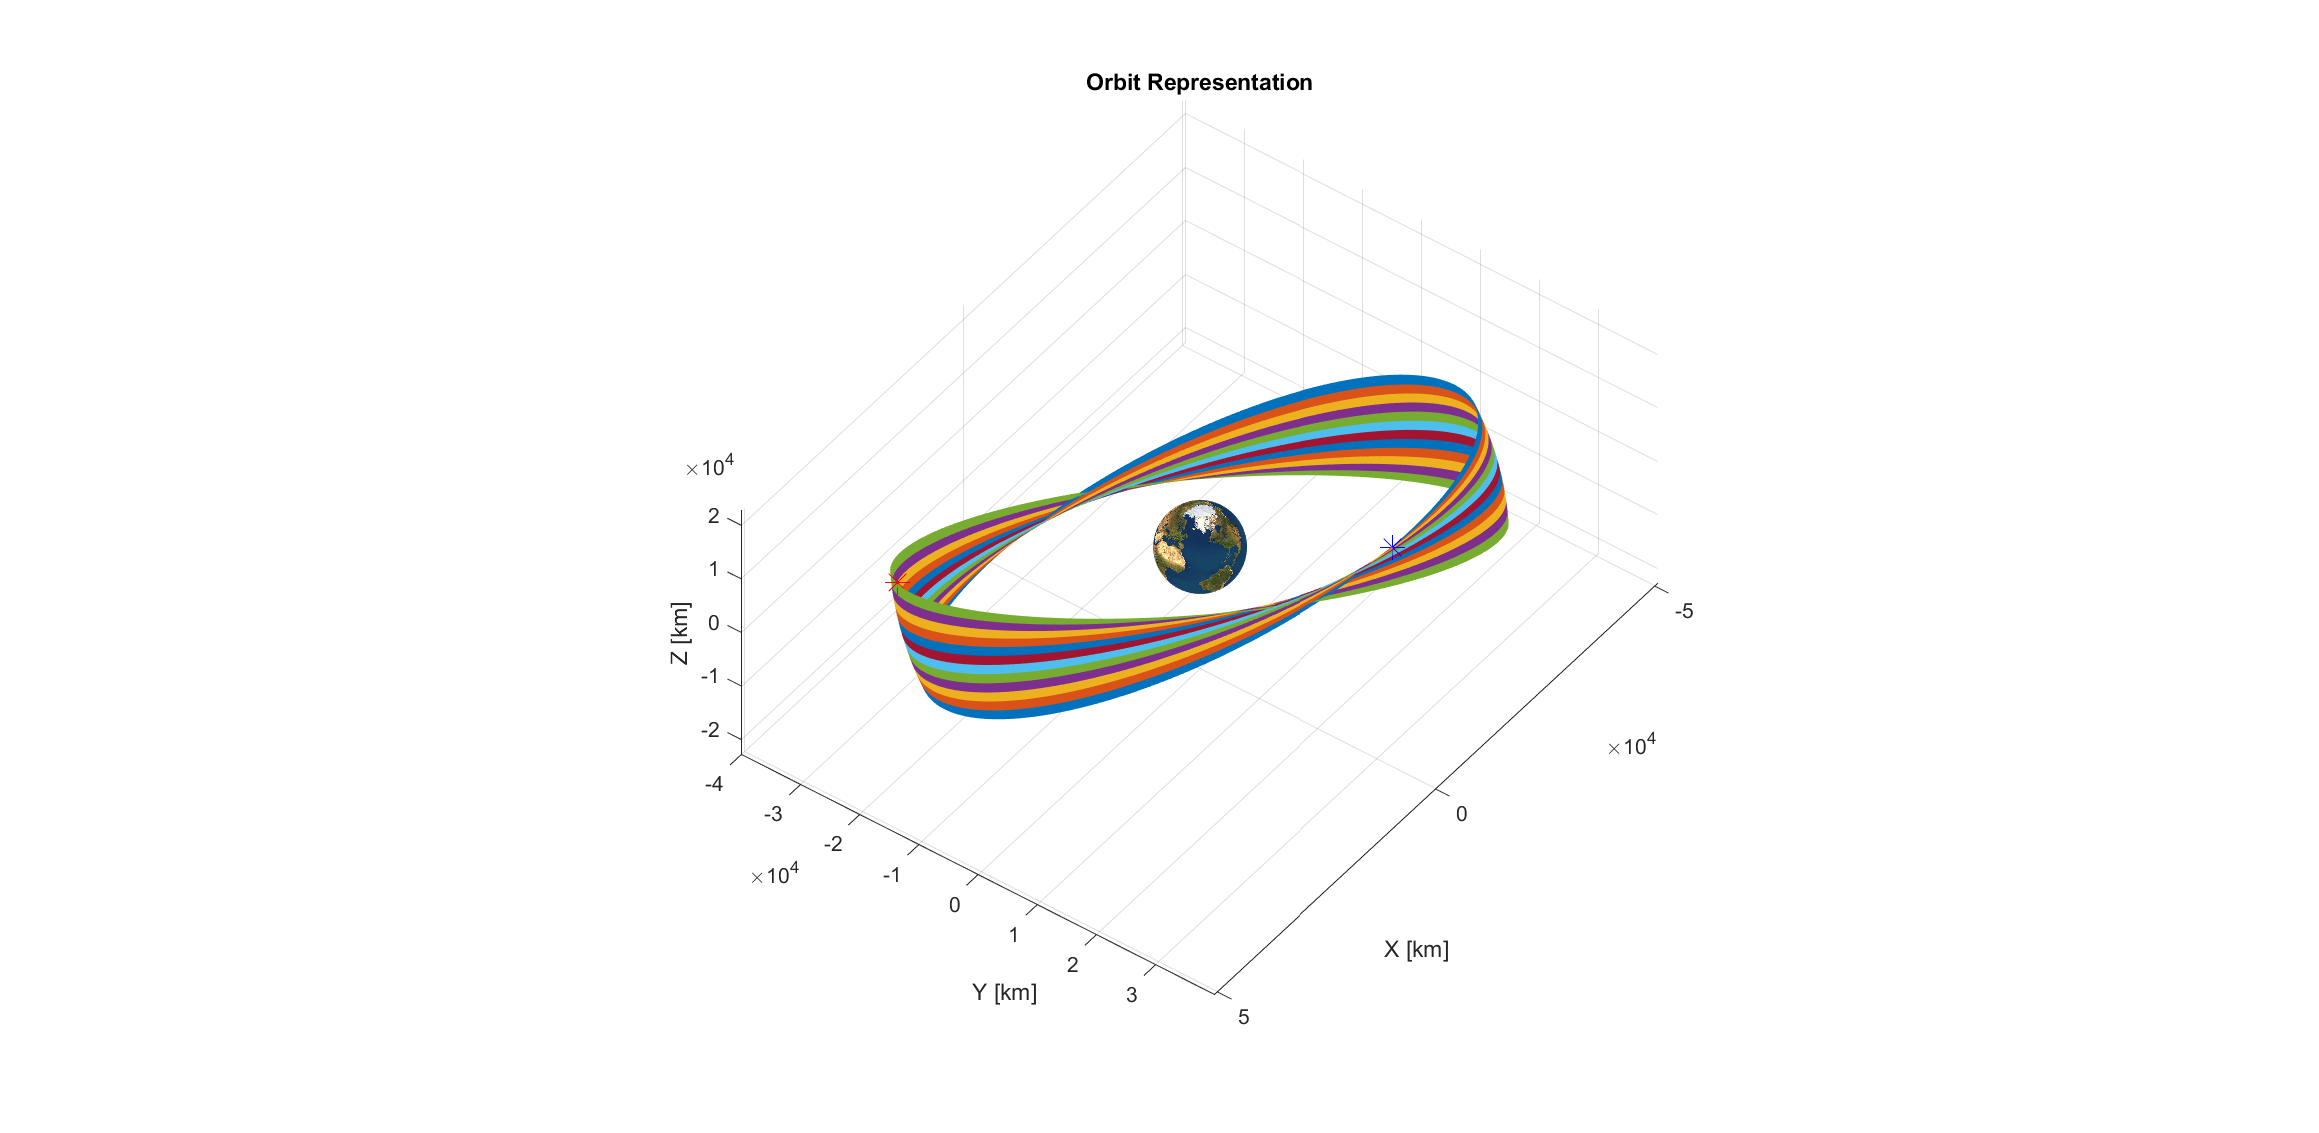
\includegraphics[width=\textwidth]{evolutionorbit2.eps}
		\caption{}
		\label{fig:1a}
	\end{subfigure}%
	\begin{subfigure}[b]{0.5\textwidth}
		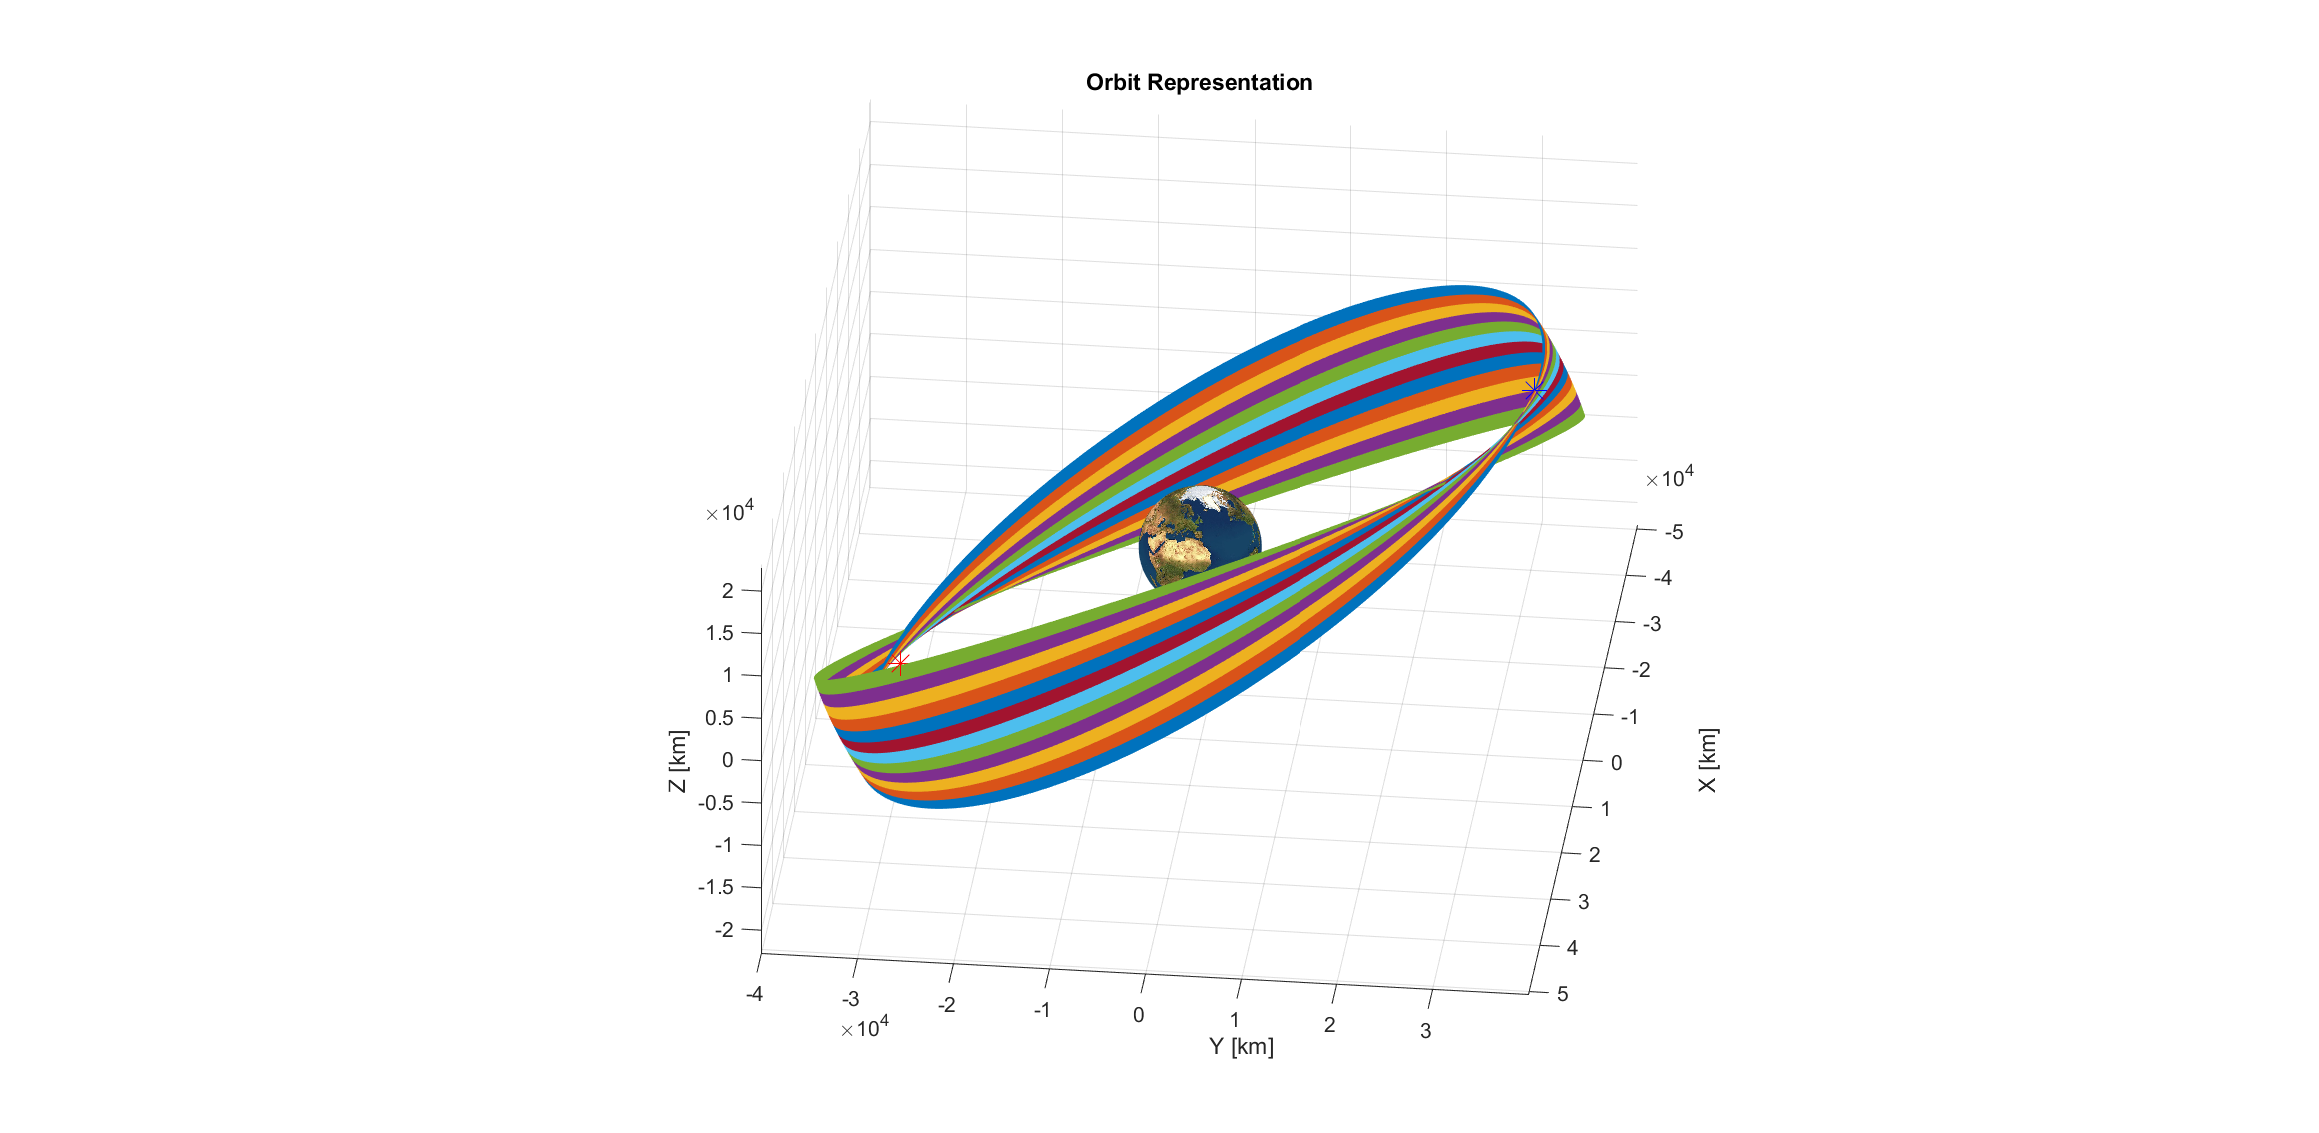
\includegraphics[width=\textwidth]{evolutionorbit3.eps}
		\caption{}
		\label{fig:1b}
	\end{subfigure}
	\caption{Orbit evolution representation in the 3D plane. Colors are used in order to let the reader understand the evolution of the orbit: in chronological order there are (\bluedashedline), (\orangedashedline), (\yellowdashedline), (\purpledashedline), (\reddashedline), (\greendashedline), (\cyandashedline), and (\magentadashedline). The initial position of spacecraft is (\textcolor{blue}{*}) and the final position of spacecraft is (\textcolor{red}{*}).
	}
\end{figure}

\subsection{Filtering} 

The filtering of results is now performed to see how the perturbations generate behaviours with different frequencies, and to retrieve the long-period and the secular evolution of the data.

\begin{figure}[H]
	\centering
	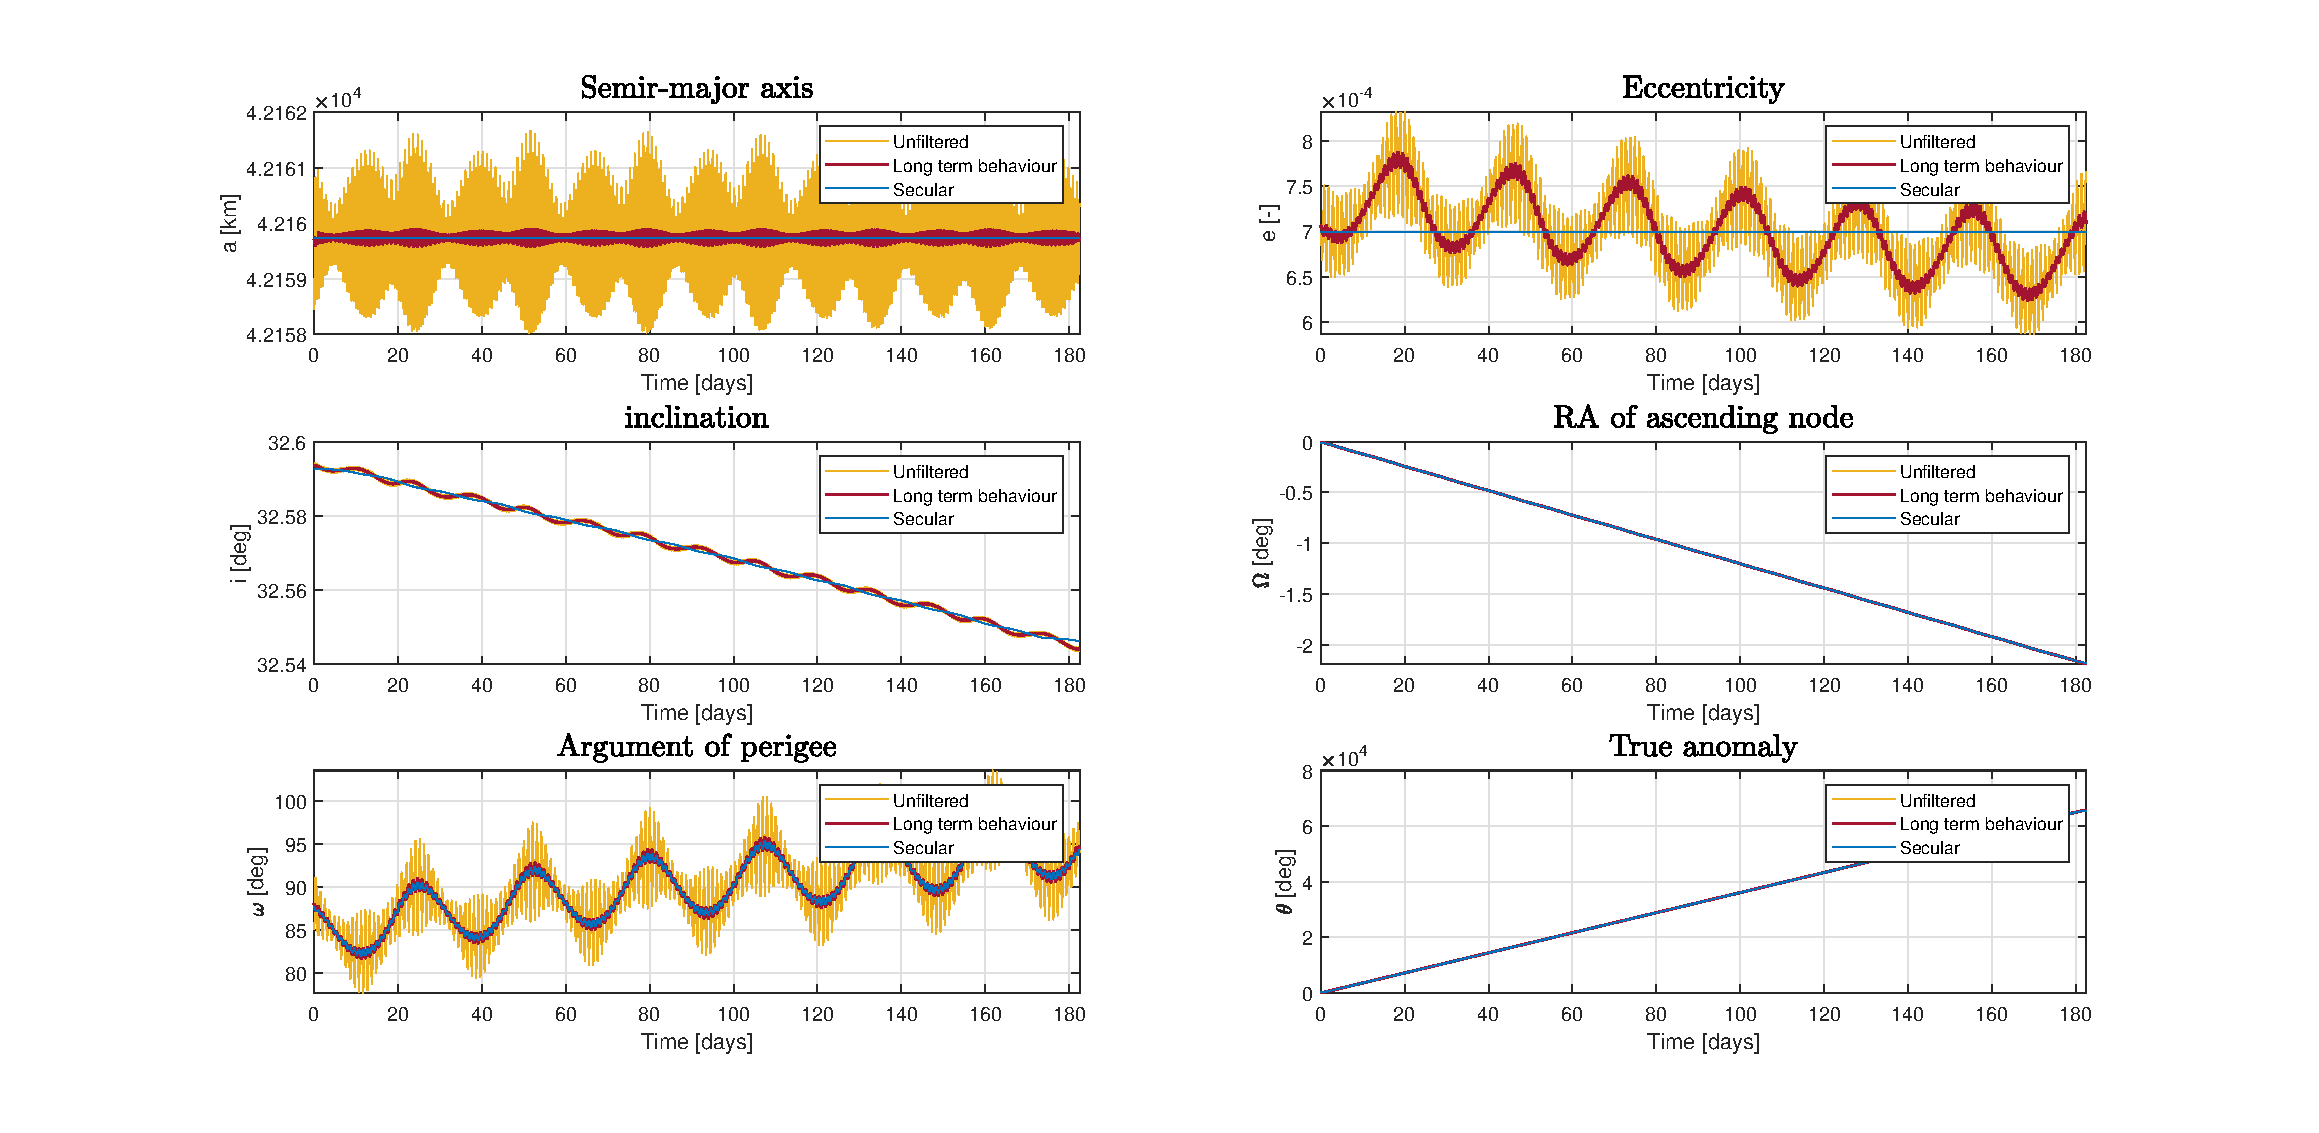
\includegraphics[width=1\textwidth]{filter0.5year.eps}
	\caption{Orbit Perturbations.}
	\label{fig:filtering}
\end{figure}

Here, long-periodic behaviour is related to moon perturbation and short-periodic perturbation is related to J2 effect. This is due to the fact that the J2 perturbation is related to the oblateness of the Earth and of the S/C’s orbit, whose period is much lower than the Moon orbit period. Two different filters are used: the filter used to remove short-term behaviour has a cut-off frequency of \(100 \, \text{days}^{-1}\), instead, the filter used to remove long-term behaviour has a cut-off frequency of \(1 \, \text{days}^{-1}\).


\section{Comparison with Real Data}

\begin{figure}[H]
	\centering
	% First row with two figures
	\begin{subfigure}[b]{0.45\textwidth}
		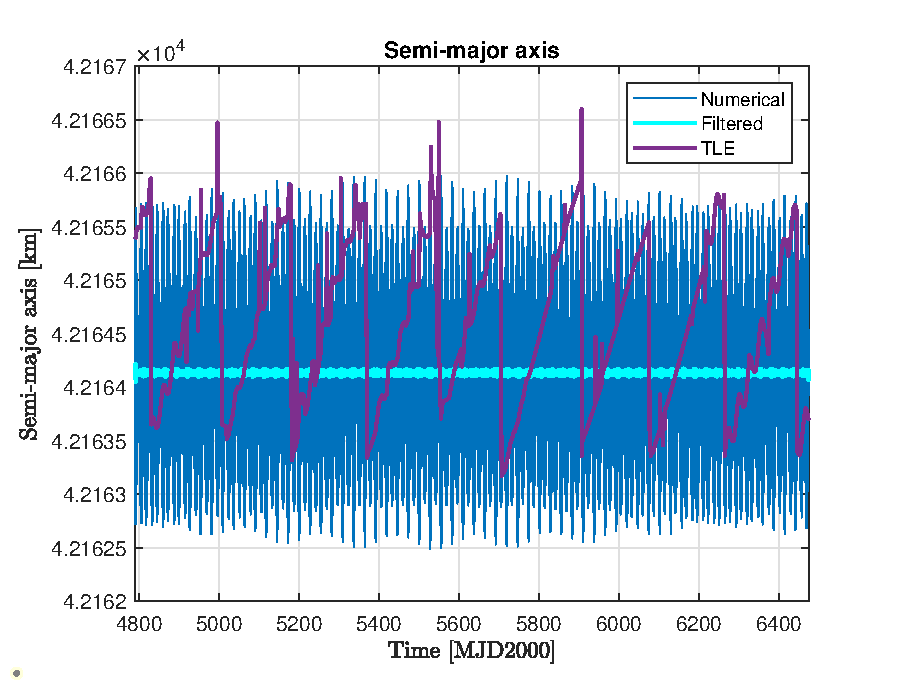
\includegraphics[width=\textwidth]{a_TLE.eps}
		\caption{}
		\label{fig:1a}
	\end{subfigure}%
    \hfill
	\begin{subfigure}[b]{0.45\textwidth}
		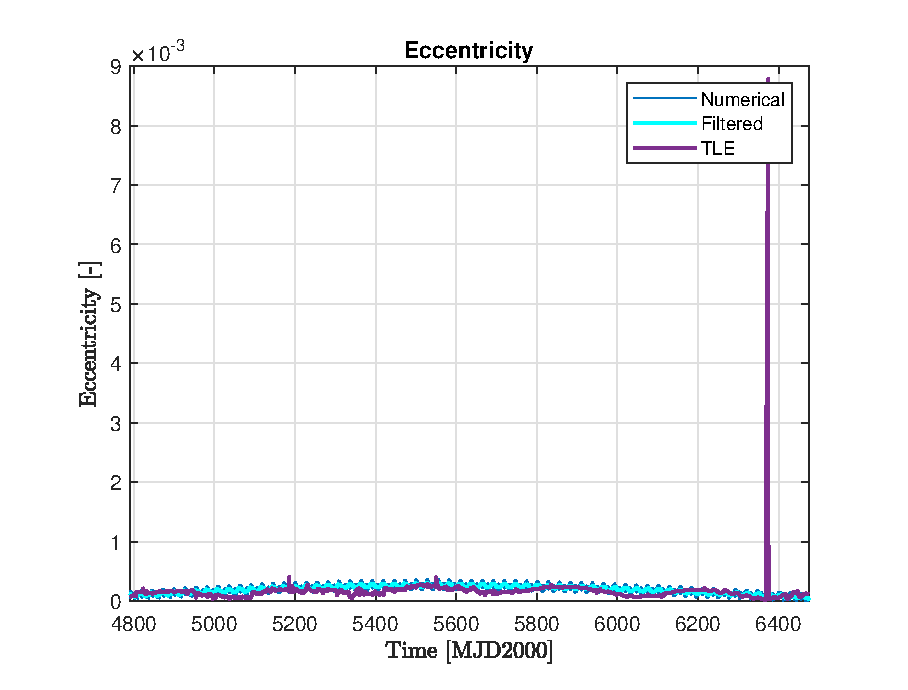
\includegraphics[width=\textwidth]{e_TLE.eps}
		\caption{}
		\label{fig:1b}
	\end{subfigure}%
	
	% Second row with two figures
	\vspace{1cm} % Adjust the vertical spacing as needed
	\begin{subfigure}[b]{0.45\textwidth}
		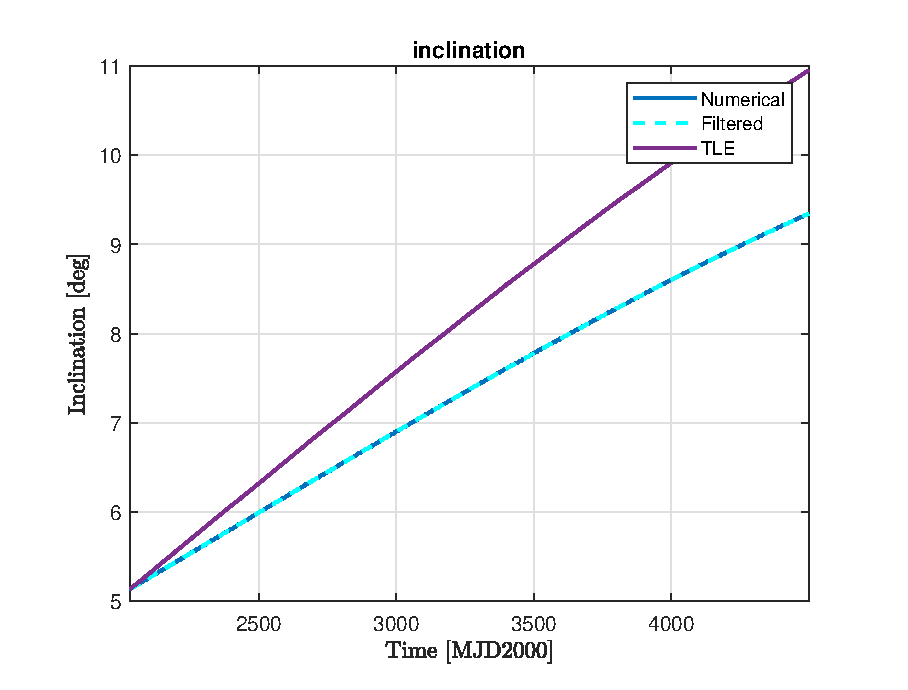
\includegraphics[width=\textwidth]{i_TLE.eps}
		\caption{}
		\label{fig:1c}
	\end{subfigure}%
    \hfill
	\begin{subfigure}[b]{0.45\textwidth}
		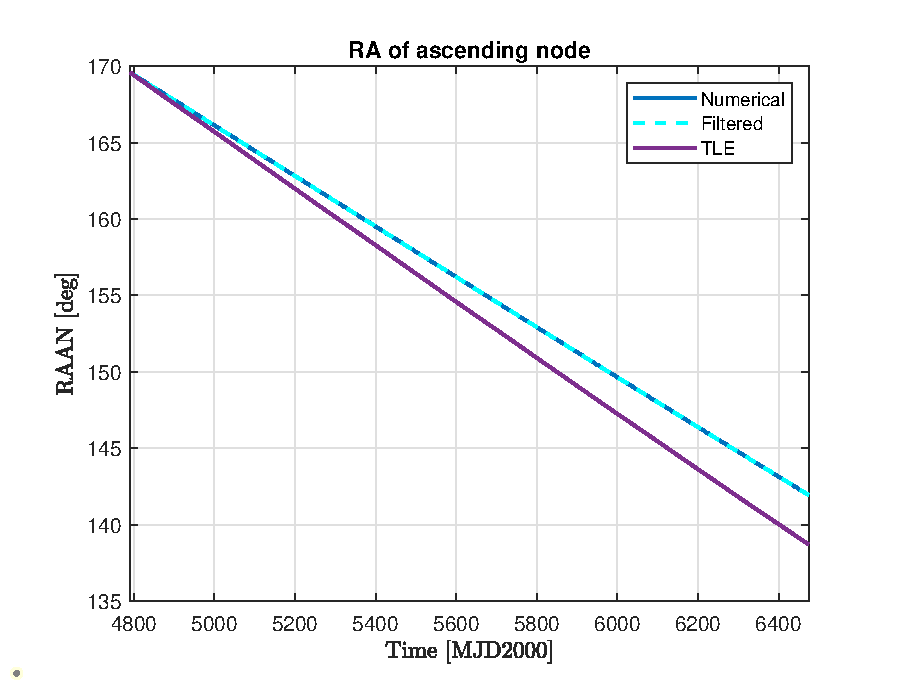
\includegraphics[width=\textwidth]{RAAN_TLE.eps}
		\caption{}
		\label{fig:1d}
	\end{subfigure}%
	
 % third row with two figures
	\vspace{1cm} % Adjust the vertical spacing as needed
	\begin{subfigure}[b]{0.45\textwidth}
		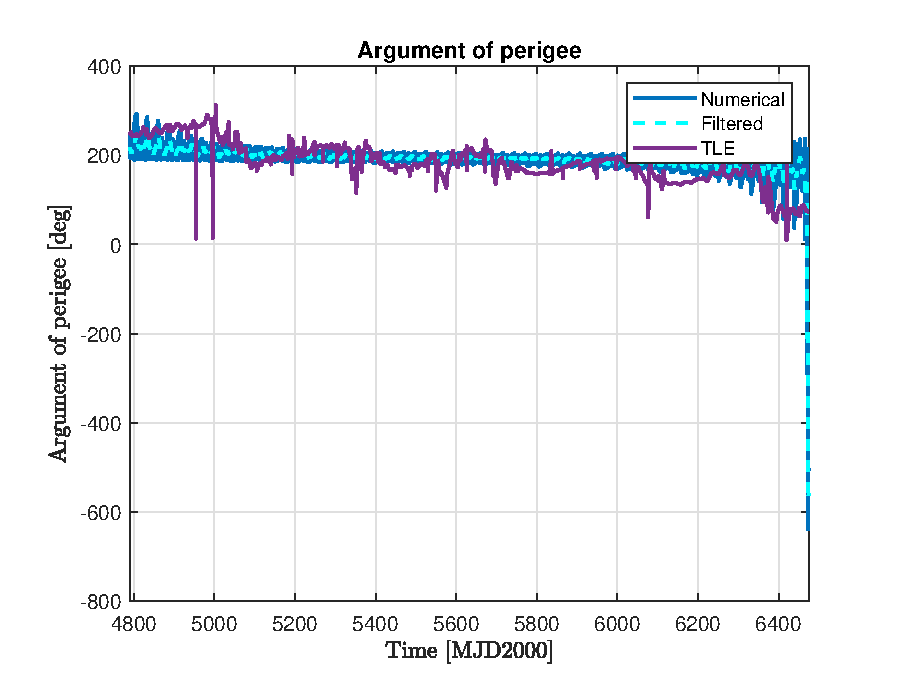
\includegraphics[width=\textwidth]{w_TLE.eps}
		\caption{}
		\label{fig:1c}
	\end{subfigure}%
	\hfill
	\begin{subfigure}[b]{0.45\textwidth}
		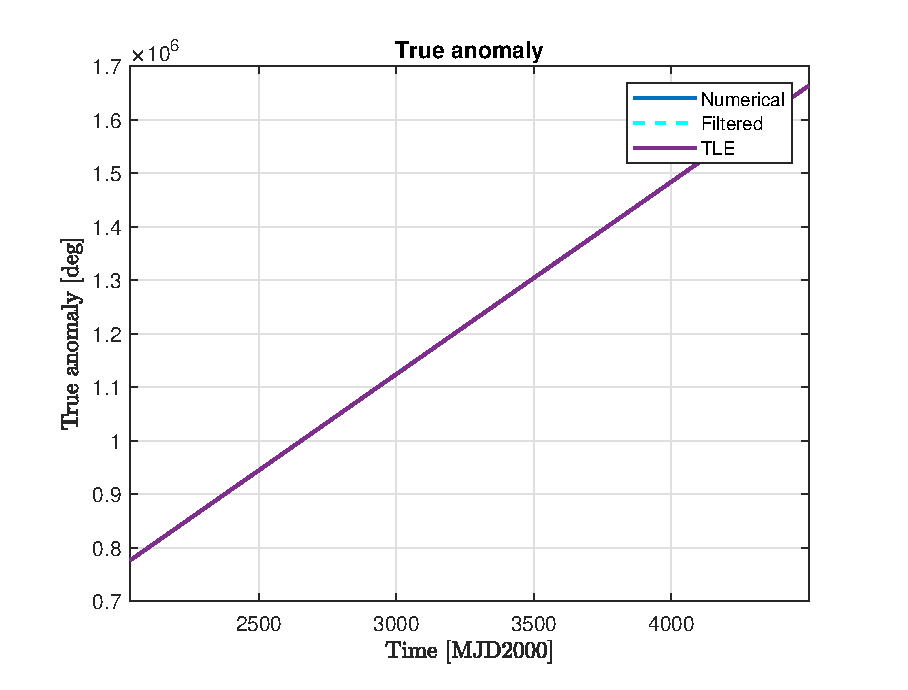
\includegraphics[width=\textwidth]{TA_TLE.eps}
		\caption{}
		\label{fig:1d}
	\end{subfigure}
	
	\caption{Numerical, filtered and TLE data
	}
\end{figure}



	
\end{document}
